\documentclass[preprint,12pt]{elsarticle}
% Elsevier's official article class. Reference style: numbered (elsarticle-num).
\usepackage{amsmath,amssymb}
\usepackage{graphicx}
\usepackage{booktabs}
\usepackage{tabularx}
\usepackage{url}
\def\UrlBreaks{\do\/\do\-\do\:\do\a\do\b\do\c\do\d\do\e\do\f\do\0\do\1\do\2\do\3\do\4\do\5\do\6\do\7\do\8\do\9}
\usepackage[hidelinks]{hyperref}
\usepackage{lineno}
\usepackage{placeins}
\linenumbers
\graphicspath{{../figures/}{figures/}}
\newcolumntype{Y}{>{\raggedright\arraybackslash}X}

\journal{Reliability Engineering \& System Safety}

\begin{document}

\begin{frontmatter}

\title{Evidence, not verdicts: what 590 public PX4 crash logs can and cannot tell a drone fleet operator}

% ---- Authors ----
\author[a]{Nagesh Chougule\corref{cor1}}
\ead{nkc.mech@coeptech.ac.in}
\author[a]{Vibhav Ambardekar}
\author[a]{Aditya Pathare}
\author[a]{Atharv Waghmare}
\author[a]{Shreyash Pawar}
\author[a]{Piyush Bhamare}
\cortext[cor1]{Corresponding author.}
\affiliation[a]{organization={Department of Mechanical Engineering, COEP Technological University},
            city={Pune}, country={India}}

\begin{abstract}\small
Flight logs are widely expected to show whether a drone crash was caused by the pilot or the aircraft. Across 590 PX4 crash logs from 479,547 flights (520 real hardware, 205 rule-evaluated, 148 modelled), we examine telemetry's evidentiary value when guarding against leakage and confounding. Confirmatory tests were declared in version control ($^\dagger$marks review additions). A fixed attribution rule reached 0.47 balanced accuracy on 112 held-out crashes (pass mark 0.70). $^\dagger$Models gave AUCs 0.41--0.50 (upper bounds $\le 0.62$); with 36 pilot-labelled crashes in the modelling sample, 80\% power requires AUC $\approx 0.65$ asymptotically (0.75 under permutation null), far below the $\approx 0.8$ needed for operational verdicts. $^\dagger$On 43 expert logs the rule was inconclusive (balanced accuracy 0.381, 95\% CrI 0.25--0.61; pilot recall 1 of 5). $^\dagger$Decomposition shows crash anticipation collapses primarily via cohort selection: evaluating the 67 multi-flight crashes against independent other-aircraft normals yields AUC 0.522 [0.413, 0.615], and uncalipered within-drone evaluation yields no detectable precursor signal in this cohort (Group-CV AUC 0.569, cluster bootstrap [0.500, 0.643]; rank test $\bar r=0.48$). Caliper matching ($|\Delta \ln(\text{duration})| \le 0.25$) lifts within-drone AUC to 0.642 ($+0.110$ on 36 airframes; 95\% paired cluster CI [+0.074, +0.238]), suggesting duration differences mask precursors in this cohort. $^\dagger$Checks were consistent with leakage (exploratory, tuning sensitivity fell from 7/9 to 1/9 without the final 10\,s, unadjusted $p=0.031$, alongside normal false alarms falling from 13\% to 5\%). Crashed drones vibrated more on older estimator metrics (mean rank 0.67, Holm $p=0.016$; newer metrics inconclusive, $p=0.25$). $^\dagger$Screening against 107 controls yielded $3.3\times$ operational lift (illustrative PPV 2.26--2.43\% at 10\% flag rate). AeroFleet~2.0 presents longitudinal evidence without automatic verdicts.
\end{abstract}

\begin{keyword}
Unmanned aircraft systems \sep Flight logs \sep Crash investigation \sep Fault diagnosis \sep Data leakage \sep Fleet assurance
\end{keyword}

\end{frontmatter}

% ===================================================================
\section{Introduction}
\label{sec:intro}

Small unmanned aircraft are now flown commercially for survey, inspection, agriculture and delivery, and the rules
that govern them place weight on records. In the European Union and the United Kingdom an operator in the specific
category must keep records of operations, maintenance and personnel for at least three years
\cite{eu2019947,easa2024ear}; India requires an accident to be reported within 48 hours \cite{india2021rules}, and
the United States within ten days \cite{faa107}. When something goes wrong, the onboard flight log is the richest
record available. Open-source log viewers, commercial fleet platforms and, more recently, machine-learning and
language-model prototypes promise to turn that log into an answer: what failed, and whether the pilot or the aircraft
was responsible \cite{duvvuru2025llm,silalahi2026droptc}.

The question matters beyond engineering curiosity. In aviation safety science, accidents are recognized as systemic,
multi-causal events involving human factors, environmental conditions and organizational influences \cite{wiegmann2003hfacs}.
Commercial warranty claims, insurance settlements and regulatory filings nevertheless frequently compress these dynamics
into a binary decision: whether the pilot or the aircraft was primarily responsible. An automatic verdict that looks
objective can carry weight it has not earned. Fleet operators face a related but different question: not why one flight
ended badly, but which of their drones are most likely to fail next and should be inspected first. A log-based method that
is good at the second task need not be good at the first, and confusing the two can mislead both investigators and maintainers.

Whether logs can deliver on either expectation has, to our knowledge, not been tested at scale against real crashes
with evaluation protocols that guard against the two known sources of optimism. First, a log that contains a crash also
contains its consequences---saturated motors, extreme attitudes and estimator errors---so a detector can learn the crash
itself rather than its cause, a form of crash-window data leakage
\cite{kaufman2012leakage,kapoor2023leakage}. Second, comparing crash flights with other operators' good flights mixes
the flight with the aircraft and the people using it, so a difference between groups need not say anything about the
flight that crashed (between-aircraft confounding). Public fault datasets are dominated by simulation or injected faults
\cite{keipour2021alfa,le2025rflymad,kabaoglu2026uavsead}, and accident statistics classify outcomes such as loss of
control rather than causes visible in a log \cite{wild2016drone,aaib2024review}; neither resource tests
whether real crash logs, evaluated under leakage-free and within-aircraft protocols, can support the attribution and
prioritization decisions that operators actually need.

The central question this paper asks of the largest public archive of real autopilot logs, PX4 Flight Review
\cite{meier2015px4,px4flightreview}, is: \textit{what evidentiary value can flight logs carry for a drone fleet
operator, once evaluation protocols guard against crash-window leakage and between-aircraft confounding?} We decompose
this into four sub-tests:
\begin{enumerate}
\item[Q1] Do configuration settings differ between crash flights and normal flights, and can that difference indicate
          who was responsible?
\item[Q2] Can a log separate crashes caused by the pilot from crashes caused by the aircraft---and does this separation
          survive expert-diagnosis validation?
\item[Q3] Once within-aircraft and between-aircraft comparisons are distinguished, which comparison retains a usable
          signal of pre-crash deterioration?
\item[Q4] Do expert diagnoses agree with uploader labels, and do automatic diagnostic checks find the faults experts
          name without benefiting from the crash window?
\end{enumerate}
Because language-model assistants are now proposed for exactly this task, we also report a controlled evaluation of
small local models used as an attribution review panel, including a test for voting-consensus manipulation.

The contributions are as follows.
(i)~A methodological decomposition isolating why apparent crash anticipation collapses: evaluating the same 67 multi-flight crash flights against independent matched normal flights from other aircraft yields an AUC of 0.522 [0.413, 0.615] (Step~4b), consistent with the collapse being driven by evaluation cohort selection rather than by within-drone baseline adjustment alone (scoring 103 multi-history crashes from the broader archive against unselected normals retains an AUC of 0.891, showing that cross-sectional models exploit between-aircraft duration and vehicle envelope confounds). Furthermore, within-drone evaluation finds no detectable precursor signal under uncalipered matching in this cohort (Group-CV AUC 0.569, 95\% cluster bootstrap CI [0.500, 0.643], pairwise mean AUC 0.592 [0.516, 0.692], rank test $\bar r=0.48$), whereas exploratory duration caliper matching ($|\Delta \ln(\text{duration})| \le 0.25$) yields an AUC lift of $+0.110$ to $+0.125$ (95\% paired cluster bootstrap CI [+0.074, +0.238] on 36 airframes), suggesting that baseline duration mismatch masks within-drone precursors in this cohort.
(ii)~We assemble, to our knowledge, a small first validation set of real-flight crash logs from public PX4 archives that pairs uploader responsibility labels
with independent expert forum diagnoses ($\kappa \geq 0.73$, 148 threads, 43 downloadable logs).
(iii)~We show that with these rules, models and labels, cross-validated classification yielded AUCs between 0.408 and 0.501
(upper 95\% bootstrap bounds 0.510--0.619); with only 36 pilot-labelled crashes in the modelling sample, 80\% power requires an AUC of roughly 0.65 under asymptotic theory (0.75 under the empirical permutation null), far below the roughly 0.8 an operational attribution verdict requires. Agreement
with expert forum diagnoses was statistically inconclusive (balanced accuracy 0.381, 95\% CrI 0.25--0.61, conservative class-averaged bound 0.19--0.73; cannot exclude agreement at the declared 0.70 pass mark; pilot recall 1 of 5).
Our prospectively declared negative result applies to the heuristic rule (balanced accuracy 0.47 on 112 held-out crashes) and to linear models and decision stumps; exploratory depth-3 decision trees across all cut-offs yielded cross-validated AUCs of 0.517 [0.392, 0.636] at $m=0$\,s, 0.594 [0.482, 0.706] at $m=2$\,s, 0.603 [0.479, 0.724] at $m=5$\,s, 0.379 [0.249, 0.524] at $m=10$\,s, 0.468 [0.331, 0.604] at $m=20$\,s, and 0.366 [0.223, 0.519] at $m=30$\,s (upper bounds near 0.73 occur only when terminal tumble telemetry is retained, dropping to 0.524 under 10\,s leakage control). Furthermore, apparent diagnostic check accuracy
is consistent with crash-window leakage (as an exploratory illustration, tuning check sensitivity fell from 7/9 to 1/9, unadjusted $p=0.031$, alongside a drop in normal false alarms from 13\% to 5\%).
(iv)~We report one partial positive screening signal: drones that later crash are rougher than matched peers on ordinary flights on older
estimator metrics (mean rank 0.67, Holm $p=0.016$); replication on newer accelerometer metrics was inconclusive
($p=0.25$, 19 sets, severely underpowered). As an exploratory illustration, screening against 107 stratum-matched fleet controls at an assumed 10\% flag rate yields an operational lift of $3.3\times$ (illustrative PPV 2.26--2.43\% [exact Bayes] across screenable and fleet base rates; 41.2--44.2 inspections per detected crash)---a maintenance
prioritization signal, not an operational warning.
(v)~We show how these results translate into design implications for fleet assurance tools that present longitudinal evidence
and rank drones without issuing automatic verdicts. Code, declarations, derived features and labels are released.

% ===================================================================
\section{Related work}
\label{sec:related}

\paragraph{Fault datasets} Table~\ref{tab:datasets} compares our data with the main public resources. ALFA provides
47 fixed-wing flights with injected engine and control-surface failures \cite{keipour2021alfa}. RflyMAD covers 5,629
multicopter fault cases with eleven fault types, of which 497 are real flights and the rest software- or
hardware-in-the-loop simulations \cite{le2025rflymad}. UAV-SEAD offers about 1,396 real PX4 logs annotated for
state-estimation anomalies \cite{kabaoglu2026uavsead}, used by later anomaly-mining work \cite{wei2026aerotsboost};
a recent testbed quantifies the discrepancies between simulated and real PX4 logs \cite{kose2026testbed}. These
resources target anomaly or fault detection under known faults. To our knowledge, none of these public resources
labels real crashes by responsibility or separates the pre-crash window from the crash.

\begin{table}[t]
\centering
\caption{Public UAV fault and anomaly data compared with this study.}
\label{tab:datasets}
\small
\begin{tabularx}{\textwidth}{@{}lYYY@{}}
\toprule
Resource & Flights & Faults or labels & Real crashes labelled by cause (to our knowledge) \\
\midrule
ALFA \cite{keipour2021alfa} & 47 fixed-wing flights & Injected engine and control-surface failures & No \\
RflyMAD \cite{le2025rflymad} & 5,629 cases (497 real) & 11 injected fault types & No \\
UAV-SEAD \cite{kabaoglu2026uavsead} & about 1,396 real PX4 logs & State-estimation anomalies (4 classes) & No \\
This study & 479,547-log index; 590 crash-rated logs; 148 expert-diagnosed threads & Uploader responsibility labels; expert causes & Yes (uploader; partly expert-checked; to our knowledge) \\
\bottomrule
\end{tabularx}
\end{table}

\paragraph{Fault detection and diagnosis} Surveys of fault detection for UAVs and robots cover model-based and
data-driven methods and stress how hard robotic diagnosis is in the field \cite{puchalski2022uav,khalastchi2018fdd}.
Causal models built from autopilot documentation have been used to find actual causes of failures in ArduPilot logs
\cite{zibaei2024causal}. A study of 569 bugs in PX4 and ArduPilot found parameter handling among the root-cause types
of drone-specific bugs \cite{wang2021autopilot}. Maintenance-oriented reliability analysis of UAVs models the passage
from partial degradation to failure \cite{petritoli2018reliability}, the view our between-drone result supports.

\paragraph{Accident analysis} Analyses of civil drone occurrences find equipment problems and loss of control
prominent \cite{wild2016drone}. Human-factors frameworks for remotely piloted aircraft (such as the Human Factors
Analysis and Classification System, HFACS) model mishaps as multi-causal sequences involving organizational influences,
environmental preconditions, and supervisory failures alongside direct operator actions \cite{wiegmann2003hfacs,tvaryanas2006hfacs}.
In operational practice, post-incident reporting and warranty claims often collapse these complex systemic interactions into
a single nominal party: pilot versus aircraft. Because such classifications depend heavily on the rater and framing,
we evaluate agreement against expert community diagnoses.

\paragraph{Language models for diagnosis} Language-model agents have been applied to simulation testing and log
analytics for small UAVs \cite{duvvuru2025llm}, and learned models to classifying problems in drone log messages for
forensics \cite{silalahi2026droptc}. Multi-agent debate has been proposed to improve the factuality of model outputs
\cite{du2024debate}, while indirect prompt injection shows that text inside data can steer model behaviour
\cite{greshake2023injection}. We test both properties on our task.

\paragraph{Methodology} Leakage, where information unavailable at prediction time enters training or evaluation, is a
known source of irreproducible machine-learning results \cite{kaufman2012leakage,kapoor2023leakage}; label noise
likewise biases evaluation \cite{frenay2014label}. In the drone-log domain we identify a domain-specific variant:
\textit{crash-window leakage}, in which the physical consequences of the crash (saturated actuators, estimator divergence,
attitude extremes) contaminate features used to evaluate pre-crash diagnostics. Matching reduces confounding in
observational comparisons \cite{stuart2010matching}, and declaring hypotheses and analysis scripts in version control
prior to running tests separates confirmatory from exploratory analysis \cite{nosek2018prereg}. We apply these ideas
together as an evaluation protocol for drone logs.

% ===================================================================
\section{Data}
\label{sec:data}

\subsection{Archive and labels}
PX4 Flight Review is a public service to which PX4 users upload onboard logs (ULog format) for plotting and sharing
\cite{px4flightreview}. We downloaded its public index on 20 October 2026: 479,547 logs (32,793,172 bytes,
SHA-256 \texttt{1bbb01c3\ldots a92d6}), of which 442,929 came from real hardware rather than simulation, from 38,320
distinct vehicle identifiers. Uploaders may rate a log. A total of 590 logs carry an uploader crash rating (402
aircraft-caused, 188 pilot-caused); Table~\ref{tab:composition} details the 520 crash-rated logs from real hardware with
duration $\ge 10$\,s and complete firmware version records. These uploader-assigned responsibility labels are not independently
verified ground truth; they reflect the uploaders' own assessments. A notable discrepancy appears between uploader ratings
and expert conclusions: while uploaders attributed 31.9\% of rated crashes to the pilot (188 of 590), forum experts blamed
the pilot in only 6.1\% of all threads (9 of 148) and 8.6\% of decided threads (9 of 105, Section~\ref{sec:experts}). Across all
148 real crash threads, download attempts yielded 43 downloadable logs from 43 distinct threads (38 aircraft-fault and 5 pilot-fault;
the remaining 105 had unhosted or expired external links). Cross-tabulating these 43 logs against archive ratings reveals that
9 carried uploader aircraft crash ratings (\texttt{crash\_sw\_hw}, with 100\% expert agreement: all 9 diagnosed as aircraft faults),
33 were unrated in the archive index (28 aircraft, 5 pilot), 1 was rated unsatisfactory (aircraft), and exactly 0 were uploaded
with a \texttt{crash\_pilot} rating. This pattern is consistent with, but not statistical evidence of, reluctance to self-identify
pilot fault: all 5 pilot logs were unrated in the index against 28 of 38 aircraft logs unrated (one-sided Fisher exact $p = 0.25$).
Across the wider set of all 148 forum threads, 14 referenced logs that carried an uploader aircraft crash rating in the archive
index (experts agreed with the aircraft fault in 11 and were unclear in 3; none blamed the pilot); 9 of these 14 threads were among
the 43 with surviving, downloadable log files (all 9 with complete expert agreement), while 5 had expired external links. This gap
may reflect selection bias in which incidents operators submit for community assistance, or a narrower definition of pilot error
among autopilot developers compared to end users. Furthermore, forum diagnoses represent informed community opinion rather than
independently verified accident inspection ground truth; original posters explicitly confirmed the diagnosis in only 47 of 94 aircraft
threads and 5 of 9 pilot threads.
Logs rated ``good'' or ``great'' served as normal flights. Logs were parsed with pyulog. We store derived features and log identifiers,
not the logs.

A ULog file contains the parameters in force when logging started, any parameter changes during logging, timestamped
messages published by the autopilot's modules, and logged text messages with a severity level. The analyses below use
the vehicle status (arming state, navigation mode, failsafe flags), attitude and body-rate topics, rate setpoints,
inertial-sensor status, actuator outputs, battery status, GPS position and the land detector. The vehicle identifier
in the index is derived from the flight controller's hardware serial number; it identifies a flight controller, which
in practice usually means one airframe, though a controller can be moved between frames.

Crash-rated logs differ from well-rated logs in composition (Table~\ref{tab:composition}): they are shorter (median
54\,s against 388\,s, partly because a crash ends the log) and spread over more firmware generations. All between-group
comparisons below therefore use either matching or within-drone designs, and we do not pool across firmware
generations where measurements differ.

\begin{table}[t]
\centering
\caption{Composition of crash-rated and well-rated logs from real hardware in the archive.}
\label{tab:composition}
\small
\begin{tabularx}{\textwidth}{@{}lYY@{}}
\toprule
 & Crash-rated & Rated good or great \\
\midrule
Logs & 520 & 21,112 \\
Median duration & 54\,s & 388\,s \\
Most frequent years & 2018 (91), 2025 (89), 2019 (87), 2017 (57) & 2018 (10,571), 2017 (5,748), 2019 (2,910) \\
Most frequent PX4 versions & 1.8 (70), 1.9 (66), 1.15 (65), 1.11 (65) & 1.7 (6,299), 1.8 (5,785), 1.6 (4,265) \\
Vehicle types & quadrotor 320, fixed wing 71, hexarotor 38 & quadrotor 19,890, fixed wing 620, hexarotor 291 \\
\bottomrule
\end{tabularx}
\end{table}

\subsection{Samples}
Figure~\ref{fig:flow} and Table~\ref{tab:samples} show how each analysis sample was drawn. We evaluate two primary classification tasks: Task A (separating crash flights from normal flights) and Task B (binary attribution of crash responsibility between drone and pilot). We distinguish two distinct
cohorts that each happen to number 148: (1) the leak-curve and attribution modeling sample of 148 crashes and 139 normal
flights at $m=0$\,s (Section~\ref{sec:methods}), and (2) the expert community sample of 148 crash discussion threads on the
PX4 forum (Section~\ref{sec:experts}). The attribution rule was evaluated on 205 crashes (93 development and 112 held-out).
All 148 crashes entering the statistical attribution models are a strict complete-case subset of these 205 crashes (100\%
overlap); 57 crashes were excluded from modeling because required ULog topics were unrecorded or the flight window before
cut-off was shorter than 10\,s. In the leak-curve and attribution modeling sample, sample sizes across cut-off margins
$m \in \{0, 2, 5, 10, 20, 30\}$\,s reflect progressive attrition as flights with duration under 10\,s before cut-off are dropped:
for Task A (crash vs.\ normal), 148 vs.\ 139 ($m=0$\,s), 142 vs.\ 137 ($m=2$\,s), 135 vs.\ 133 ($m=5$\,s), 114 vs.\ 130
($m=10$\,s), 100 vs.\ 128 ($m=20$\,s), and 89 vs.\ 124 ($m=30$\,s); for Task B (drone vs.\ pilot responsibility among crashes),
112 vs.\ 36 ($m=0$\,s, $n=148$), 106 vs.\ 36 ($m=2$\,s, $n=142$), 101 vs.\ 34 ($m=5$\,s, $n=135$), 87 vs.\ 27 ($m=10$\,s,
$n=114$), 73 vs.\ 27 ($m=20$\,s, $n=100$), and 63 vs.\ 26 ($m=30$\,s, $n=89$). A constant complete-case subset of 213 flights
(89 crashes and 124 normal flights; 63 drone and 26 pilot crashes) with pre-crash duration $\ge 40$\,s was evaluated across
all six margins without attrition.

Initial cross-sectional samples for Q1 and Q2 selected flights with PX4 1.10 or newer and at least 5\,s of flight; normal
flights were matched to crashes on vehicle type and drawn from vehicles without any crash rating. For the longitudinal
within-drone and between-drone tests (Q3b, Q3c), only the eligible case count ($n=12$), not any outcome or feature data, was
inspected before deciding to lift the firmware restriction to avoid sample starvation; flights were instead strictly matched
within each drone's firmware generation and measurement source. For the within-drone test every crash with a vehicle identifier
and at least three earlier non-crash flights of 30\,s or more was eligible (101 crashes; up to the five most recent earlier
flights each). For the between-drone test each crashed drone was matched with up to two drones without any crash-rated log
that shared the flight-controller hardware, the PX4 major.minor version and the vehicle type (66 matched sets, 124 control
slots drawn from 107 unique non-crash control drones, three randomly chosen flights each, seed 7). Control drones were sampled
without replacement within each matched set. The three exposure flights of a crashed drone were its most recent non-crash flights
dated on or before the crash; flights on the crash day were included in the declared test because the archive does not give their
order within a day, and removed in a sensitivity analysis.

Not all selected flights enter every test. In the within-drone candidate pool (101 crashes with earlier flights), 34 crashed drones
were dropped because they lacked multiple valid flights or had duration under 10\,s before cut-off, leaving 67 multi-flight drones
(372 total flights: 67 crash and 305 earlier flights). Among these 372 flights, 55 individual flight logs could not be read or had
under 10\,s before cut-off; requiring that crash and earlier flights share the same measurement source left 61 analysed drones for
vibration, and restricting to rotary-wing vehicles with rate setpoints left 46 analysed drones for rate tracking. In the between-drone
sample (66 matched sets), 71 flights were unreadable or too short; a drone's value requires at least two readable flights, and case
and controls must share the measurement source, leaving 60 analysed sets for vibration and 47 for tracking. In the between-drone sample,
124 matched control slots contributed 372 flights ($124 \times 3$), distinct from the 372 flights (67 crash flights and 305 earlier flights)
evaluated in the within-drone longitudinal model.

\begin{figure}[t]
\centering
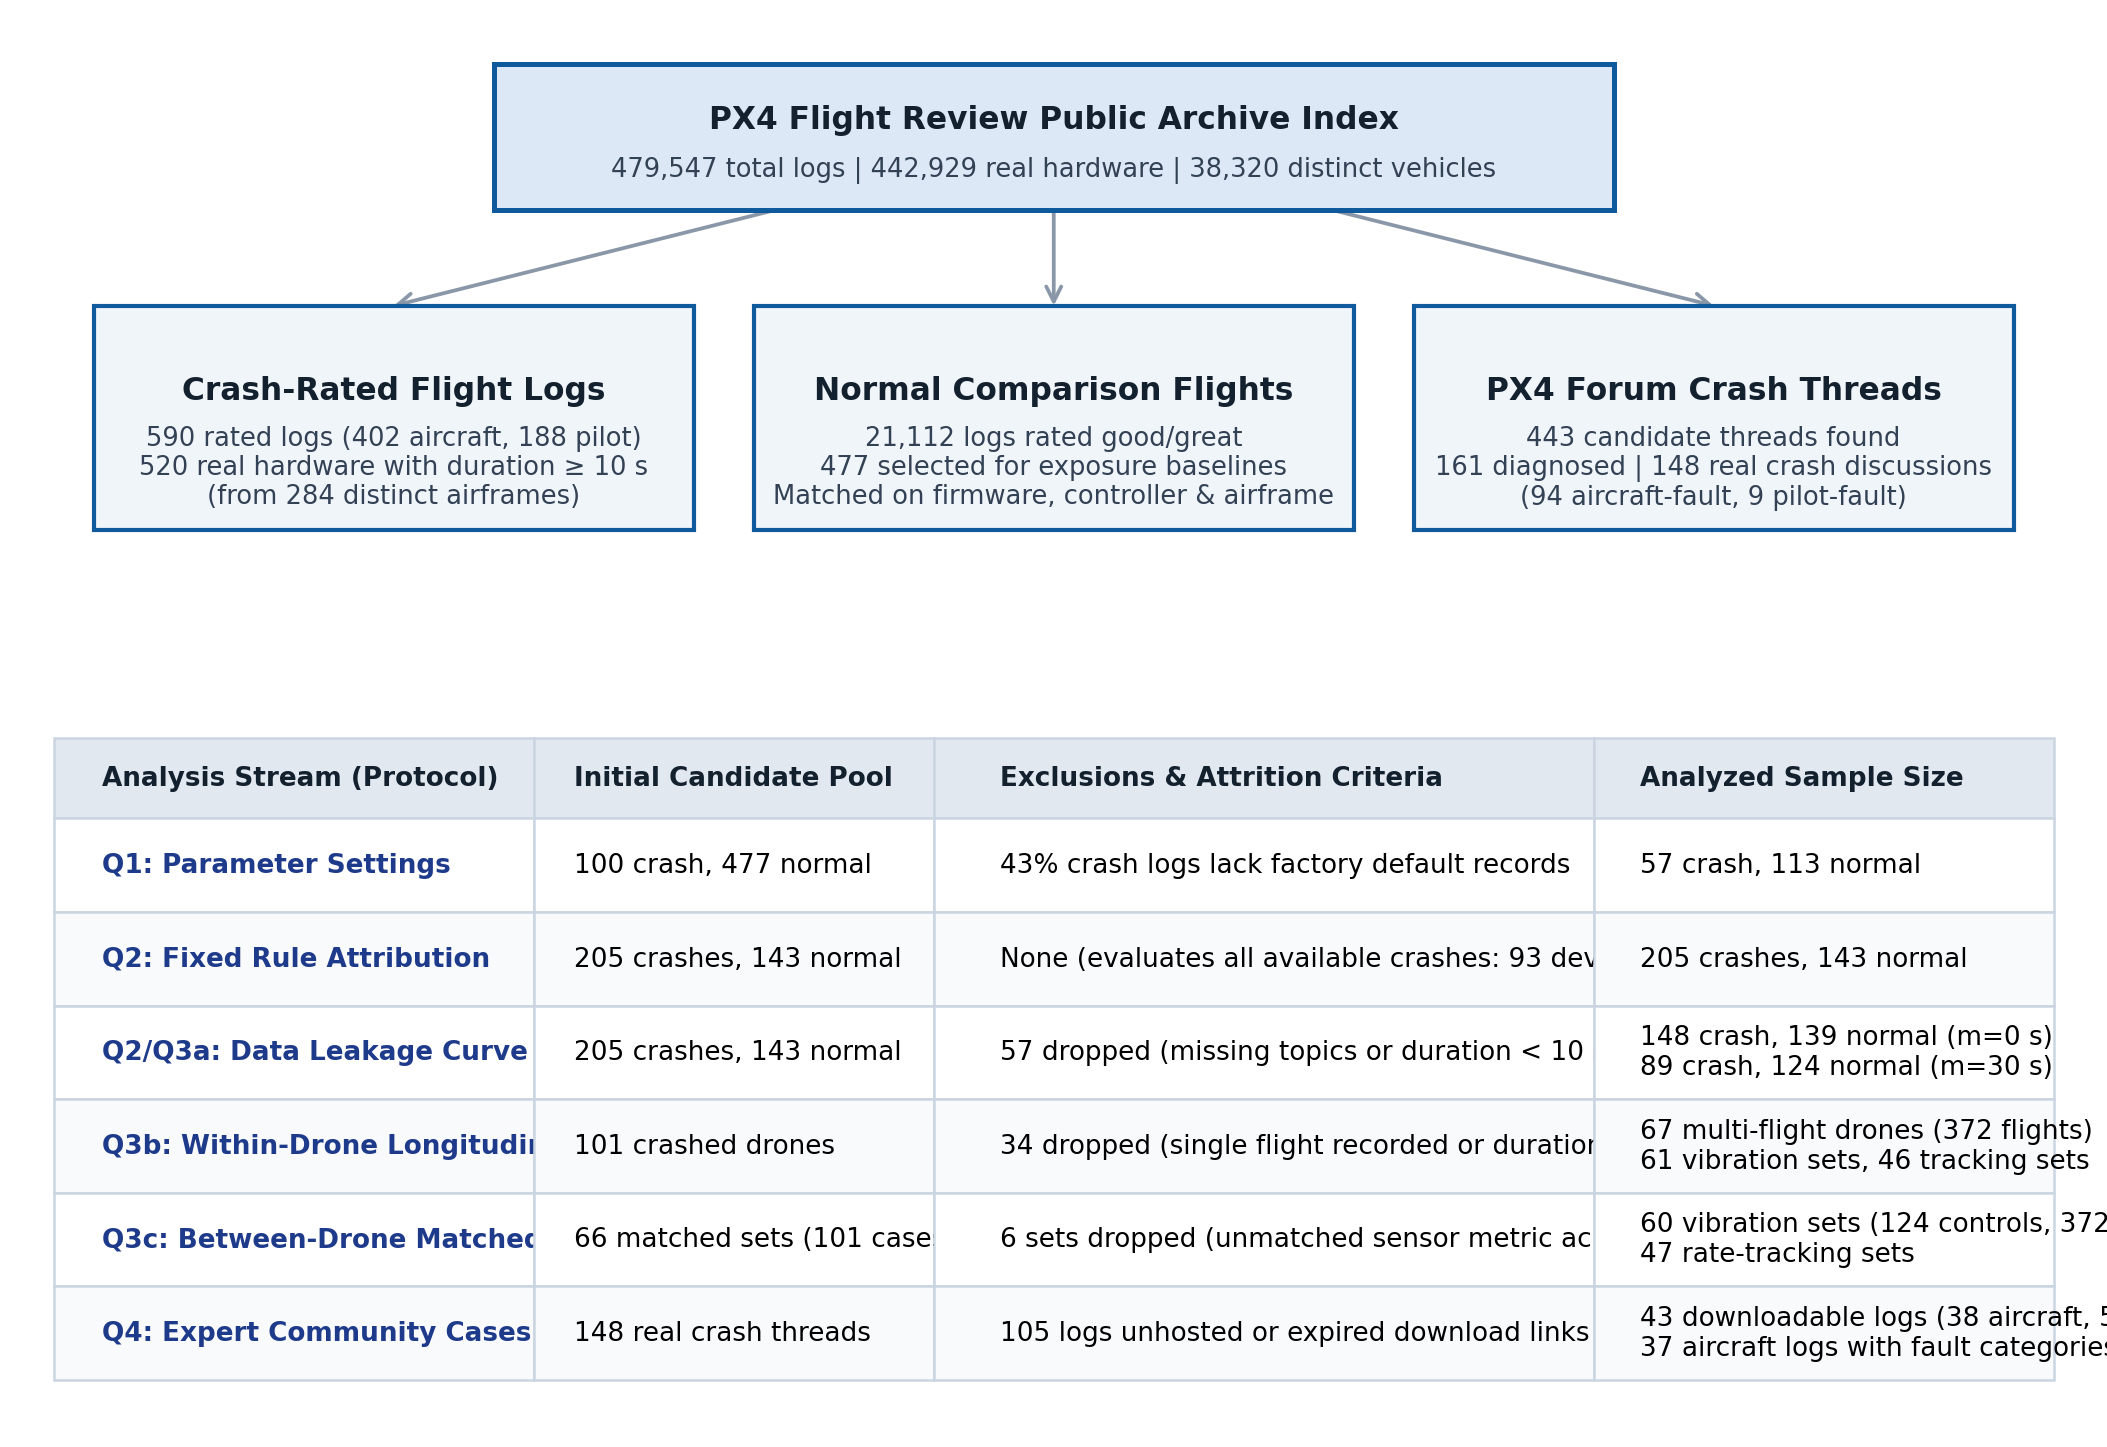
\includegraphics[width=\textwidth]{fig_study_flow.png}
\caption{From the public index to each analysis. Counts are logs unless stated.}
\label{fig:flow}
\end{figure}

\begin{table}[t]
\centering
\caption{Analysis samples and evaluation cohorts.}
\label{tab:samples}
\small
\begin{tabularx}{\textwidth}{@{}lYYl@{}}
\toprule
Sample & Crashes & Comparison & Question \\
\midrule
Settings & 100 (57 with default records) & 477 normal (113 with default records) & Q1 \\
Development crashes & 93 analysed & -- & Q2 rule \\
Held-out crashes & 112 analysed & 143 normal (full logs) & Q2 replication \\
Leak-curve set & 148 at $m=0$\,s (89 at $m=30$\,s) & 139 normal (124 at $m=30$\,s) & Q2 model, Q3a \\
Constant-subset leak curve & 89 crashes ($\ge 40$\,s duration) & 124 normal ($n=213$ constant across margins) & Q2 model, Q3a \\
Within-drone rank test & 101 selected (61 and 46 analysed) & 475 earlier flights of the same drones & Q3b \\
Within-drone predictive model & 67 multi-flight drones (67 pre-crash) & 305 earlier flights of same drones ($n=372$) & Q3b \\
Between-drone matched sets & 66 matched sets (60 and 47 analysed) & 124 matched drones, 372 flights & Q3c \\
Expert forum cases & 148 real crash threads & 43 logs downloadable (38 aircraft, 5 pilot) & Q4 \\
\bottomrule
\end{tabularx}
\end{table}

\subsection{Expert diagnoses}
We searched the PX4 discussion forum for threads that link a Flight Review log and mention a crash (443 threads, 410
with a log link). For the 161 threads with a reply from PX4 staff, the development team or a member at the
forum's highest trust levels (148 of them describing a real crash), we recorded the expert's conclusion (aircraft, pilot, both, unclear, no diagnosis), the
cause named, who gave it, whether the original poster confirmed it, and the sentence stating the diagnosis. Recording
was AI-assisted and reviewed by an author; 123 of 124 recorded sentences were found verbatim in their thread by script.
A second author then coded all threads blind to the first recording, with the same categories; a script confirmed
that 150 of 151 coded rows quoted their own thread or recorded no diagnosis. On the 147 threads both coded,
agreement (Cohen's kappa, 95\% bootstrap interval) was 0.81 (0.71--0.88) for the expert's conclusion, 0.73
(0.65--0.81) for the cause and 0.79 (0.69--0.88) for whether the poster confirmed it, above the declared pass mark
of 0.60. The two coders settled the 45 threads that differed on conclusion or cause by discussion, which changed 13
labels; counts and tests below use the settled labels, and the first recording led to the same conclusions (both
are in the repository).
The searches combined the Flight Review host names with the words crash, crashed, flyaway, fell, flipped and lost
control, and every returned thread was retrieved through the forum's public interface. A reply counted as expert when
its author was marked as staff, belonged to the development team group or held one of the forum's two highest trust
levels. Only public posts were used; usernames and post text are not redistributed.

% ===================================================================
\section{Methods}
\label{sec:methods}

\subsection{Declared test protocols}
\label{sec:protocol}
The public archive index was downloaded on 20 October 2026. For each confirmatory test, the hypothesis, sample selection, features, statistic, and pass mark were declared and committed to version control before the analysis it governs was run (Table~\ref{tab:registration}). Where a test reused logs already downloaded for an earlier test, the protocol records it as declared before running, not before download (exploratory additions added during revision are marked with $^\dagger$). Unlike third-party timestamped registries (such as the Open Science
Framework), commit timestamps in self-hosted git remain author-controlled until an independent snapshot is indexed; the git commit
history establishes an immutable cryptographic SHA-1 chain in version control, and archived snapshots have been deposited in
Software Heritage (\nolinkurl{swh:1:rev:bad06ff1256865c7e63d44389aac174e0281291d}, \nolinkurl{swh:1:rev:bbdd0420de4547ac7d67b84165292a46237b604d},
\nolinkurl{swh:1:rev:624dd694e0d207dd9c44b1c9550faaf04453bc56}, and \nolinkurl{swh:1:rev:3a9aa89417fa9ea2a2334e3a4794e2358fb713ee}) alongside
the repository's git commit hashes (including \texttt{eb463b5} for the decomposition), and will be minted into a Zenodo archive DOI upon publication. One amendment was data-dependent:
after observing that the firmware filter of the within-drone test left only 12 eligible cases under the initial $\ge 1.10$ filter
(without inspecting any outcome data), the firmware filter was removed and a fallback for older firmware was added. One coding error was corrected after a first run (logs whose CPU-load record
lacked the load field were being skipped); no threshold changed. Secondary sensitivity analyses and diagnostic
evaluations added during peer review are explicitly designated as exploratory and documented with commit hashes in
Section~\ref{sec:posthoc}.

\begin{table}[t]
\centering
\caption{Pre-declared confirmatory protocol registration schedule and version control provenance. All commits occurred prior to execution of the governed analysis. Commit timestamps reflect author-controlled local git records (IST) prior to Software Heritage archival.}
\label{tab:registration}
\small
\setlength{\tabcolsep}{3.0pt}
\begin{tabularx}{\textwidth}{@{}l p{0.34\textwidth} c c c c@{}}
\toprule
Test & Focus / Hypothesis & Commit & Commit date & Run date & Status \\
\midrule
Q1 & Protections disabled (Fisher exact) & \texttt{63bc72e} & 2026-10-20 & 2026-10-20 & Confirmatory \\
Q2 (dev) & Fixed attribution rule (BA $\ge 0.70$) & \texttt{af6fab2} & 2026-10-20 & 2026-10-20 & Confirmatory \\
Q2 (held) & Held-out rule replication (BA $\ge 0.70$) & \texttt{4475c8c} & 2026-10-20 & 2026-10-20 & Confirmatory \\
Q4 ($m=0$) & Expert fault checks on full window & \texttt{0c8ee47} & 2026-10-20 & 2026-10-20 & Confirmatory \\
Q4 ($m=10$) & Expert fault checks at $m=10$\,s & \texttt{0c8ee47} & 2026-10-20 & 2026-10-20 & Confirmatory \\
Q3a & Crash window leak curve ($\Delta \ge 0.10$) & \texttt{d5d56c7} & 2026-10-23 & 2026-10-23 & Confirmatory \\
Q3b & Within-drone rank test ($\bar r > 0.50$) & \texttt{8b417d2} & 2026-10-23 & 2026-10-23 & Confirmatory \\
Q3c & Between-drone rank test ($\bar r > 0.50$) & \texttt{d7a6574} & 2026-10-23 & 2026-10-23 & Confirmatory \\
Replication & Newer-metric accelerometer vibration & \texttt{2148644} & 2026-10-24 & 2026-10-24 & Confirmatory \\
Coding & Inter-rater blind agreement ($\kappa \ge 0.60$) & \texttt{21af373} & 2026-10-24 & 2026-10-24 & Confirmatory \\
\bottomrule
\end{tabularx}
\end{table}

\subsection{Crash moment and analysis window}
For rotary-wing aircraft the crash moment $t_c$ is the first time after take-off at which the tilt
$\theta=\arccos\left(1-2(q_x^2+q_y^2)\right)$, computed from the attitude quaternion, exceeds $60^\circ$; for fixed-wing
aircraft, and when no such tilt occurs, it is the end of the armed period. Normal flights use the end of the armed
period. Take-off is the first sample after arming at which the land detector reports the vehicle airborne. An analysis
with cut-off $m$ uses the window from take-off to $t_c-m$ and is skipped if the window is shorter than 10\,s. Because
normal flights include the complete descent, landing and disarm sequence while crash windows terminate at impact or
tilt, this introduces an inherent windowing asymmetry that contributes to differences in duration and whole-window
aggregates.

\subsection{Features}
Table~\ref{tab:features} defines the features. Vibration is not measured the same way across firmware generations:
newer logs report an accelerometer vibration metric, older ones an estimator vibration estimate. Comparisons are
therefore only made between flights measured with the same source, and the source is recorded with every value. The
rate-tracking error falls back to the attitude message's body rates when the angular-velocity topic is absent.

\begin{table}[t]
\centering
\caption{Features computed on each analysis window.}
\label{tab:features}
\small
\begin{tabularx}{\textwidth}{@{}lY@{}}
\toprule
Feature & Definition \\
\midrule
Rate-tracking error & RMS of commanded minus measured body rate, roll and pitch (rad\,s$^{-1}$; rotary wing) \\
Tilt (p95) & 95th percentile of tilt angle (deg) \\
Vibration (p95) & 95th percentile of the accelerometer vibration metric, or of the estimator vibration estimate on older firmware \\
Clipping rate & accelerometer clipping events per second \\
Motor saturation & share of time with any motor output at 95\% or more (rotary wing) \\
Battery minimum & lowest reported remaining charge (\%) \\
Voltage sag & (start voltage $-$ minimum voltage) / start voltage \\
Poor GPS & share of time with horizontal accuracy above 5\,m or fewer than 6 satellites \\
Failsafe & 1 if a failsafe was active at any time \\
Manual share & share of time in a pilot-flown mode (manual, altitude, position, acro, stabilised) \\
Stick deflection (p95) & 95th percentile of the larger roll or pitch stick deflection \\
\bottomrule
\end{tabularx}
\end{table}

\subsection{Tests}
\paragraph{Q1 settings} For logs that carry the firmware's record of default values, a protection was counted as
disabled when its value differed from the default and switched it off (for example a failsafe action of ``none'').
Crash and normal logs were compared with Fisher's exact test.

\paragraph{Q2 attribution} Task B is defined as the binary attribution of crashes between pilot and aircraft fault (contrasted with Task A, which evaluates separating crash flights from normal flights).
The declared rule labelled a crash ``aircraft'' if any of eight signs fired before $t_c$ (a critical battery warning
or remaining charge below 10\%; any motor at 95\% or more for at least 1\,s in the last 10\,s; more than 50 clipping
events; poor GPS in a GPS-dependent mode; a failure-detector flag; an error-level message; CPU load above 95\%; an
active failsafe), otherwise ``pilot'' if the mode at $t_c$ was pilot-flown, otherwise ``unknown''. The pass mark was a
balanced accuracy of at least 0.70 on decided cases, answering at least 60\% of crashes and being wrong on at most 20\%.
A model-based check used L2-regularised logistic regression on all features ($\lambda=1$, standardised inputs, median
imputation within training folds), evaluated by stratified five-fold cross-validation repeated five times and summarised
by the ROC AUC \cite{hanley1982roc}. As an exploratory check on non-linear threshold effects, single-split decision stumps were evaluated alongside logistic regression. We also evaluated depth-3 decision trees across all cut-offs ($m \in \{0, 2, 5, 10, 20, 30\}$\,s), which yielded cross-validated AUCs of $0.517$ [0.392, 0.636] at $m=0$\,s, $0.594$ [0.482, 0.706] at $m=2$\,s, $0.603$ [0.479, 0.724] at $m=5$\,s, $0.379$ [0.249, 0.524] at $m=10$\,s, $0.468$ [0.331, 0.604] at $m=20$\,s, and $0.366$ [0.223, 0.519] at $m=30$\,s (1,000 flight-level bootstrap resamples). Upper confidence bounds near 0.73 occur specifically when terminal tumble telemetry is included ($m \le 5$\,s); removing the final 10\,s reduces the upper bound to 0.524, confirming that non-linear decision trees also fall within chance under leakage control. Because they exhibited high fold instability and were not pre-declared, they were not retained for the primary benchmark.

The signs were chosen before the analysis to cover common failure modes of PX4 multirotors: power, propulsion,
vibration, navigation, software and failsafes. The pilot rule was deliberately simple: if no aircraft sign fired and
the vehicle was in a mode in which the pilot controls attitude or position directly, the crash was attributed to the
pilot. The rule was fixed before it was run on any crash log; only the list of message types available in the logs had
been inspected.

\paragraph{Q3a crash window} The same model separated crash from normal flights at cut-offs $m\in\{0,2,5,10,20,30\}$\,s.
We declared that the AUC would fall by at least 0.10 between $m=0$ and $m=10$\,s if crash consequences drove it.

\paragraph{Q3b and Q3c rank tests} For a crashed drone $i$ with value $x_{i0}$ and comparison values
$x_{i1},\dots,x_{in_i}$, the scaled rank is
\begin{equation}
r_i=\frac{1}{n_i}\sum_{j=1}^{n_i}\mathbf{1}\left[x_{ij}<x_{i0}\right],
\end{equation}
which is 0 when the crashed drone has the lowest value and 1 when it has the highest; ties count against the
hypothesis. A rank statistic was chosen for three reasons: the two vibration sources have different units and scales,
so only orderings are comparable across drones; the number of comparisons differs between drones, which the exact null
handles directly; and the distributions are skewed, with a few very rough flights, which would dominate a mean
difference. In the within-drone test (Q3b) $x_{i0}$ is the crash flight, cut 10\,s before $t_c$, and the comparisons
are the same drone's earlier flights, each cut 10\,s before the end of its armed period. In the between-drone test (Q3c) $x_{i0}$ is the median over the crashed drone's
three most recent pre-crash flights and the comparisons are the medians of the matched controls. Under no difference
each $r_i$ is uniform on $\{0,1/n_i,\dots,1\}$ with mean 0.5, and $\bar r$ estimates the probability that the crashed
drone exceeds a comparison, the quantity estimated by the Mann--Whitney statistic \cite{mann1947test}. One-sided
$p$-values come from 100,000 draws of this exact null; 95\% confidence intervals from 10,000 bootstrap resamples of
drones \cite{efron1993bootstrap}. For the proportion of sets in which the crashed drone is the roughest, the expected
null rate depends on the mix of set sizes: among the 60 analysed vibration sets, 35 had two matched controls (null
probability $1/3$) and 25 had one control (null probability $1/2$), giving an exact Poisson-binomial expected null
proportion of $(35 \times \frac{1}{3} + 25 \times \frac{1}{2})/60 = 40.28\%$ (null mean 24.167, SD 3.745). For duration
adjustment in sensitivity analysis, $\log(\text{vibration})$ was regressed on $\log(\text{flight duration})$ within each
measurement source across all exposure flights, and the rank test was repeated on the residuals. Each test had two
primary features (vibration, rate-tracking error) at $\alpha=0.025$.

\paragraph{Q4 expert diagnoses} Expert conclusions were compared with uploader labels. Fixed deterministic checks for
the five physical failure modes named by experts were evaluated:
(i)~\textit{Tuning}: combined roll and pitch rate-tracking RMS error $> 0.30$\,rad/s over at least 50 samples;
(ii)~\textit{Vibration}: total accelerometer clipping counts $> 50$ or 95th-percentile \texttt{accel\_vibration\_metric} $> 30$\,m/s$^2$;
(iii)~\textit{GPS/Compass}: \texttt{mag\_test\_ratio} $> 1.0$ in \texttt{estimator\_status} for $\ge 1.0$\,s cumulative, or horizontal position error $\text{eph} > 5$\,m or satellites $< 6$ for $\ge 5.0$\,s cumulative while in a GPS-dependent mode;
(iv)~\textit{Motor/ESC}: any motor output at $\ge 95\%$ authority (or PWM $\ge 1950$\,$\mu$s) for $\ge 1.0$\,s cumulative;
(v)~\textit{Battery}: battery warning level $\ge 2$ (critical/emergency) or state of charge $< 10\%$.
Checks were declared useful if they fired on at least 50\% of logs with that diagnosis and at most 10\% of normal flights,
evaluated first on the full window ($m=0$\,s) and then with the final 10\,s removed ($m=10$\,s).

\paragraph{Language-model panel} The panel tested a design proposed for advisory diagnosis: several reviewers, each
restricted to one slice of evidence (navigation, pilot inputs, GPS, battery, settings), vote on a fixed list of six
causes and must cite numbered facts extracted from the log. Robustness was evaluated by replacing one reviewer with an
adversary arguing for a chosen wrong cause, and planting hostile strings in uploader-controlled fields. Full details are
provided in Section~\ref{sec:lm_summary}.

\paragraph{Multiplicity} Seven confirmatory tests produce $p$-values. Holm's procedure \cite{holm1979} is reported over
all seven in addition to each test's declared $\alpha$.

% ===================================================================
\section{Results}
\label{sec:results}

\subsection{Configuration settings (Q1)}
Of 57 crash logs and 113 normal logs carrying a firmware-default record, 29 (51\%) and 52 (46\%) had at least one
protection disabled relative to the default (Fisher $p=0.63$). Pilot-caused crashes had a protection disabled more
often than aircraft-caused ones: 14 of 20 (70\%) against 15 of 37 (41\%), an observed difference of $+29.5$\% (95\% CI
$3.9$--$55.0$\%, odds ratio 3.42, Fisher's exact two-sided $p=0.052$). This contrast is exploratory, not part of the pre-declared confirmatory family, and does not
reach statistical significance unadjusted (Fisher's exact two-sided $p=0.052$). Furthermore,
default parameter records were present only on newer firmware (missing for 43\% of the 100 crash logs); on the 57
available cases, treating disabled protections as a pilot-attribution classifier yields a sensitivity of 70.0\%, a
specificity of 59.5\%, and a balanced accuracy of 0.647, below the declared 0.70 pass mark. None of 100 crash logs
changed a safety-critical or flight-limit setting during the flight.

\subsection{Attributing a crash to the pilot or the aircraft (Q2)}
\label{sec:attribution}
The fixed rule reached a balanced accuracy of 0.57 on 93 development crashes (35\% wrong) and 0.47 on 112 held-out
crashes (47\% wrong), against the declared 0.70, and labelled 39\% of 143 normal flights as aircraft faults
(Table~\ref{tab:tests}). The signs fired at similar rates whichever party the uploader blamed
(Fig.~\ref{fig:signs}): motor saturation in 23\% of aircraft-caused and 29\% of pilot-caused crashes (1\% of normal
flights), battery warnings in 15\% and 18\% (3\%). Error messages and failsafes were no more frequent in crashes than
in normal flights. Two signals noticed after the development run did not replicate on held-out crashes: accelerometer
clipping (24\% against 8\%, $p=0.045$) and manual mode at the crash (18\% against 10\%, $p=0.165$).

In Task B, sample sizes decline across margins as flights under 10\,s are excluded: 112 drone and 36 pilot crashes
at $m=0$\,s ($n=148$), 106 vs.\ 36 at $m=2$\,s ($n=142$), 101 vs.\ 34 at $m=5$\,s ($n=135$), 87 vs.\ 27 at $m=10$\,s ($n=114$),
73 vs.\ 27 at $m=20$\,s ($n=100$), and 63 vs.\ 26 at $m=30$\,s ($n=89$). On the full sample ($n=148$ at $m=0$\,s, 75.7\% drone-blamed),
pooled cross-validated logistic regression yielded an ROC AUC of 0.408 (bootstrap SE 0.062, 95\% CI 0.288--0.530, upper 95\% bound 0.510) at $m=0$\,s,
0.422 (SE 0.072, 95\% CI 0.283--0.566, upper bound 0.542) at $m=10$\,s ($n=114$), and 0.501 (SE 0.073, 95\% CI 0.358--0.645, upper bound 0.619)
at $m=30$\,s ($n=89$). Evaluated on the constant complete-case sample of 89 crashes (63 drone, 26 pilot; 70.8\% drone-blamed) plotted in
Fig.~\ref{fig:leak}, pooled cross-validated logistic regression yielded an AUC of 0.466 (bootstrap SE 0.072, 95\% CI 0.325--0.607, upper bound 0.584)
at $m=0$\,s, 0.489 (SE 0.074, 95\% CI 0.343--0.633, upper bound 0.611) at $m=10$\,s, and 0.501 (SE 0.073, 95\% CI 0.358--0.645, upper bound 0.619)
at $m=30$\,s.

To calibrate whether these below-chance AUCs represent an inverted physical signal or finite-sample noise, we computed a 1,000-iteration
permutation null distribution on Task B by randomly shuffling crash attribution labels: the null distribution had mean 0.497
(SD 0.090) with an empirical 95\% interval of 0.313--0.660. The permutation null used the same pooled statistic (mean 0.497), so the below-chance
values are not a bias of the statistic; rather, with 36 pilot-labelled crashes against 112 drone crashes in the modelling sample, below-chance
point estimates reflect finite-sample variance under class imbalance. The empirical permutation standard deviation (0.090) is wider than the theoretical
asymptotic standard error of the Wilcoxon statistic ($\text{SE}_{\text{null}} = \sqrt{(36+112+1)/(12 \times 36 \times 112)} \approx 0.0555$).
Repeating the permutation null with fixed scores across 10,000 label permutations yields an empirical standard deviation of 0.055 (matching asymptotic theory within $\pm 0.001$), which is consistent with fold-refitting variance explaining the wider cross-validation null (SD 0.090). Under the theoretical asymptotic SE (0.056), an AUC of roughly 0.65 is detectable at 80\% power ($\alpha=0.05$,
$z_{0.80}+z_{0.975} = 2.802 \times 0.0555 \approx 0.156$ above chance). Under the empirical cross-validation permutation null (SD 0.090, the relevant null for the cross-validated logistic models evaluated here), the 97.5th percentile
of 0.660 represents only $\approx 50\%$ detection power, and 80\% power requires an AUC of roughly 0.75 ($0.50 + 2.802 \times 0.090 = 0.752 \approx 0.75$). The observed cross-validated
bootstrap upper bounds were 0.510--0.619. An operational attribution verdict would need an AUC of about 0.8 or higher, which these models
do not approach. If an operator requires not merely statistical separation from chance but confirmation that performance excludes a mediocre baseline ($\text{AUC} \le 0.80$) via a 95\% confidence lower bound under an operational target of 0.85 ($0.85 - 1.96 \times \text{SE} \ge 0.80 \implies \text{SE} \le 0.0255$), sample sizing requires at least 250 independently verified pilot-fault crashes (with matching aircraft cases, $\text{SE}_{\text{asymp}} \approx 0.021$), far beyond the 36 available in the modelling sample. We therefore report that these rules, models and labels give no usable attribution signal under the evaluated setup, not that attribution is fundamentally impossible.
Evaluating depth-1 decision stumps on Task B yielded similar results: AUC of 0.430 at $m=0$\,s (bootstrap SE 0.062, 95\% CI 0.310--0.551,
upper bound 0.534), and 0.413 at $m=10$\,s (SE 0.069, 95\% CI 0.281--0.548, upper bound 0.528). Evaluating depth-3 decision trees across cut-offs yielded pooled cross-validated AUCs of 0.517 [0.392, 0.636] at $m=0$\,s, 0.594 [0.482, 0.706] at $m=2$\,s, 0.603 [0.479, 0.724] at $m=5$\,s, 0.379 [0.249, 0.524] at $m=10$\,s, 0.468 [0.331, 0.604] at $m=20$\,s, and 0.366 [0.223, 0.519] at $m=30$\,s (1,000 flight-level bootstrap resamples; earlier exploratory development reported mean fold AUCs of $0.595 \pm 0.130$ at $m=0$\,s and $0.621 \pm 0.105$ at $m=5$\,s, which reflect fold-averaging rather than pooled out-of-fold scoring). Because confidence intervals across $m=0..5$\,s broadly overlap, fluctuations between margins represent sampling noise rather than structured trajectory trends; at $m \ge 10$\,s, upper confidence bounds contract to 0.524, providing no evidence of non-linear separation once the terminal window is excluded.

\begin{figure}[t]
\centering
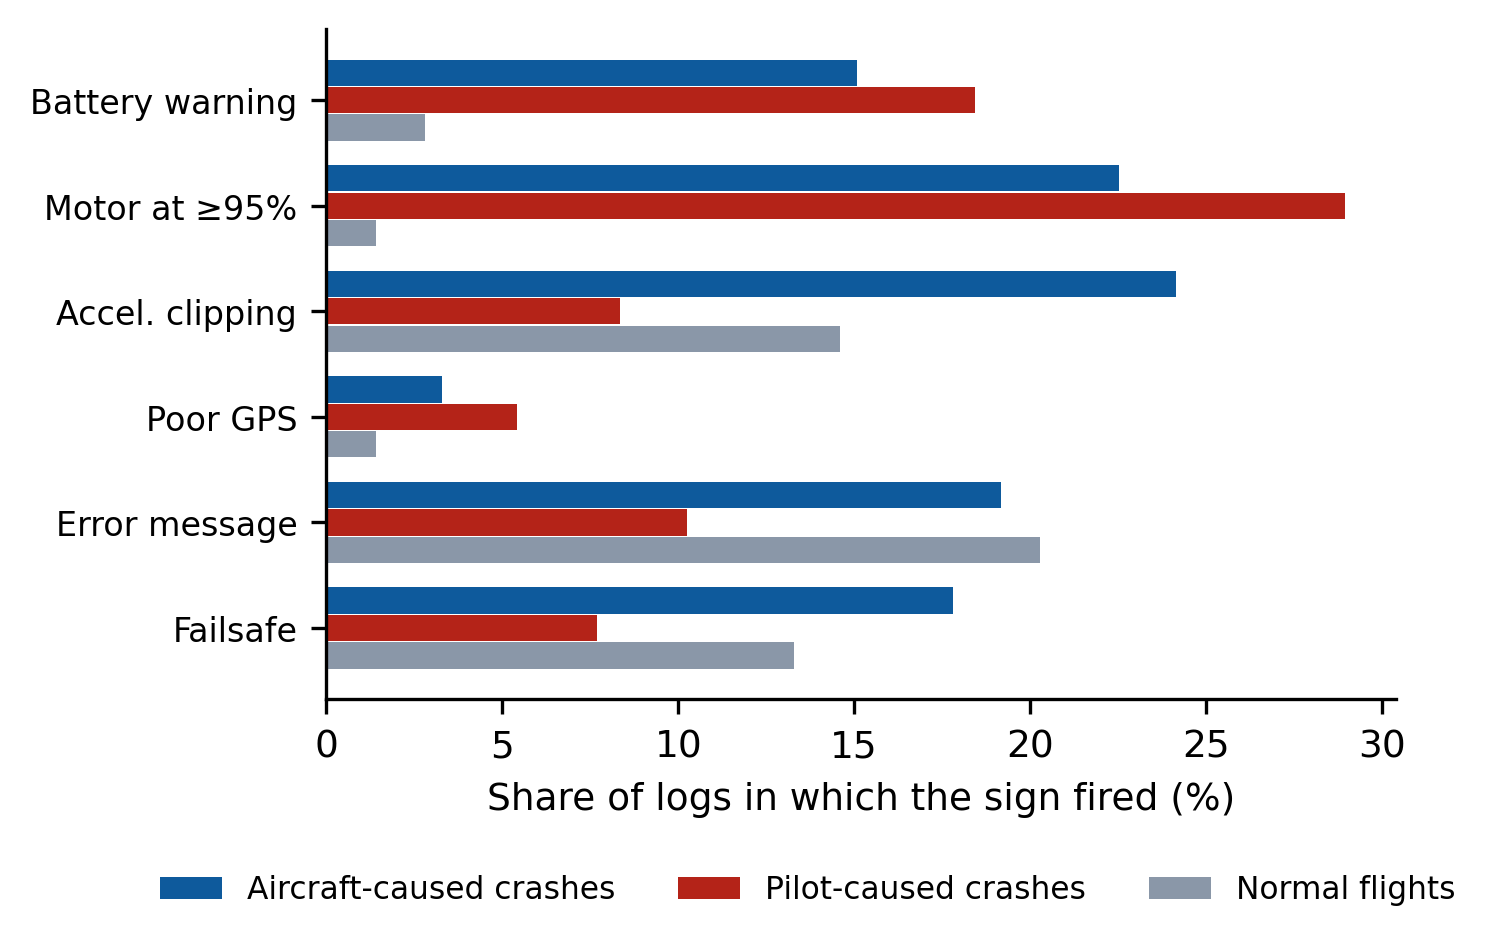
\includegraphics[width=0.78\textwidth]{fig_sign_rates.png}
\caption{How often each aircraft-fault sign fired in held-out crashes, by uploader label, and in normal flights.}
\label{fig:signs}
\end{figure}

\begin{table}[t]
\centering
\caption{Confirmatory tests, their declared pass marks and outcomes. Holm adjustment over the seven $p$-valued tests.}
\label{tab:tests}
\small
\begin{tabularx}{\textwidth}{@{}p{0.31\textwidth}p{0.24\textwidth}cY@{}}
\toprule
Test (declared criterion) & Result & Holm $p$ & Outcome \\
\midrule
Protections disabled, crash vs normal & 51\% vs 46\%, $p=0.63$ & 1.00 & No difference \\
Attribution rule, dev. (BA $\geq 0.70$) & BA 0.57, 35\% wrong & -- & Failed \\
Attribution rule, held-out & BA 0.47, 47\% wrong & -- & Failed \\
Clipping, aircraft vs pilot ($p<0.025$) & 24\% vs 8\%, $p=0.045$ & 0.27 & Not supported \\
Manual mode, pilot vs aircraft ($p<0.025$) & 18\% vs 10\%, $p=0.165$ & 0.73 & Not supported \\
AUC drop from 0 to 10\,s ($\geq 0.10$) & 0.88 to 0.87 & -- & Not supported \\
Within-drone vibration ($p<0.025$) & $\bar r=0.48$, $p=0.67$ & 1.00 & Not supported \\
Within-drone tracking ($p<0.025$) & $\bar r=0.50$, $p=0.47$ & 1.00 & Not supported \\
Between-drone vibration ($p<0.025$) & $\bar r=0.67$, $p=0.0023$ & 0.016 & Supported on older metric only; replication inconclusive \\
Between-drone tracking ($p<0.025$) & $\bar r=0.57$, $p=0.15$ & 0.73 & Not supported \\
Expert-fault checks, $m=10$\,s ($\geq 50\%$, $\leq 10\%$) & best: vibration 3/5 vs 11\% & -- & None met \\
\bottomrule
\end{tabularx}
\end{table}

\subsection{The crash window (Q3a)}
\label{sec:window}
\label{sec:confounding}
In the primary declared sample, crash flights were separated from normal flights with a cross-validated AUC of 0.88
(SD 0.01) at $m=0$\,s ($n=148$ crashes, 139 normal flights), 0.88 at $m=2$\,s (142 vs.\ 137), 0.88 at $m=5$\,s (135 vs.\ 133),
0.87 (SD 0.01) at $m=10$\,s (114 vs.\ 130), 0.86 at $m=20$\,s (100 vs.\ 128), declining to 0.86 at $m=30$\,s (89 vs.\ 124);
the declared drop of 0.10 was not observed (observed drop of 0.01). To evaluate whether this apparent stability was an artefact of sample attrition as shorter
flights dropped out at larger margins, we evaluated the cross-validation on the fixed constant subset of 213 flights
with duration $\ge 40$\,s (89 crashes, 124 normal flights; plotted in Fig.~\ref{fig:leak}) across all six margins. On this
constant sample, model AUC declined smoothly from 0.895 (SD 0.007) at $m=0$\,s to 0.876 at $m=2$\,s, 0.873 at $m=5$\,s,
0.868 at $m=10$\,s (a drop of 0.027), 0.862 at $m=20$\,s, and 0.864 at $m=30$\,s. The absence of a large drop in Task A AUC (0.895 to 0.868)
indicates that the cross-sectional model does not rely primarily on transient crash-impact telemetry. Instead, classification is likely
influenced by flight envelope differences and airframe characteristics that correlate with duration (Table~\ref{tab:features_auc}).
Although flight duration was deliberately excluded from the 11 normalized model features, duration alone separates crash from normal flights
with an AUC of 0.662 at $m=0$\,s (crash median 71.0\,s vs.\ normal median 169.0\,s) and 0.634 at $m=10$\,s, and correlates significantly with
several normalized features: longer flights exhibit larger 95th-percentile tilt ($\rho=+0.470$ at $m=0$\,s, $+0.484$ at $m=10$\,s), greater
voltage sag ($\rho=+0.321$ and $+0.357$), and larger stick deflections ($\rho=+0.363$ and $+0.233$), while shorter flights show higher rate-tracking
errors ($\rho=-0.248$ at $m=0$\,s). The absence of a large collapse holds on identical flights, confirming that changing sample composition
across cut-offs did not mask a collapse.

Leakage was nevertheless present for individual physical checks. The rate-tracking feature alone fell from an AUC of 0.81
to 0.69 as the crash was excluded, while vibration stayed between 0.72 and 0.77 (Table~\ref{tab:features_auc}). Evaluating sign firing rates across margins on 148 crashes and 139 normal flights illustrates the physical mechanism: accelerometer clipping in crashes fell from 26.4\% ($m=0$\,s) to 16.7\% ($m=10$\,s, a 37\% relative drop), while in normal flights it remained baseline at 4.3\% $\to$ 3.8\%. Failsafe activation in crashes dropped from 13.5\% to 8.8\% at $m=10$\,s and 6.0\% at $m=20$\,s, while in normal flights it remained steady at $\sim 13$--14\% (standard return-to-land and disarm triggers). Motor saturation in crashes declined from 45.9\% to 41.2\% (and in normal flights from 18.7\% to 14.6\%), reflecting exposure window truncation alongside impact saturation. A fixed tuning check that found 10 of 12
candidate expert-diagnosed tuning faults (7 of 9 on paired surviving logs) with the crash included found only 1 of 9 once
the last 10\,s were removed (Section~\ref{sec:experts}).

Crucially, the high cross-sectional model separation (AUC 0.88) does not demonstrate unconfounded anticipation of an
impending crash: crash and normal flights differ fundamentally in duration (median 54\,s against 388\,s in the broader archive;
71\,s vs.\ 169\,s in the complete-case sample), firmware era distribution, and operational flight envelope. Table~\ref{tab:features_auc}
gives the single-feature AUCs. Values below 0.5 indicate features that are lower in crash flights: crash flights reached lower tilt
and smaller stick deflections over the whole flight than normal flights, consistent with short, aborted or cautious testing flights.
Table~\ref{tab:decomposition} reports a step-by-step decomposition isolating what drives the cross-sectional separation. Grouping
cross-validation folds by vehicle ID (Step~1) on the cross-sectional sample yields virtually identical separation (AUC 0.884 vs.\ 0.883);
because crash airframes and control airframes originate from disjoint operators, vehicle-grouped cross-validation cannot remove vehicle-level
separation by design. Removing the final 10\,s or 30\,s on the constant cohort of 213 flights (Steps~2 and 3) similarly leaves the AUC essentially unchanged
(0.860 [0.802, 0.910] and 0.874 [0.822, 0.920], with flight-level bootstrap intervals confirming no substantial drop), while removing tilt and stick boundary features (Step~4) reduces AUC modestly to 0.831. Thus, vehicle grouping folds, crash-window cuts, and boundary feature pruning do not explain the cross-sectional gap. Instead, evaluating the exact same 67 multi-flight crash flights against independent matched normal flights from other aircraft (strictly excluding the 67 airframe UUIDs, matched 2:1 on vehicle type; Step~4b) collapses the model AUC to 0.522 [0.413, 0.615]. This is consistent with the collapse being driven by cohort selection across evaluation samples rather than by within-drone baseline adjustment alone. To test whether the 0.88 cross-sectional separation was an artifact carried solely by single-history crashes (vehicles with no earlier flights in the archive: maiden flights, bench tests), we scored single-history crashes ($n=45$) and multi-history crashes ($n=103$) from the Step~0 sample separately against the 139 normal flights. Both subsets yielded high cross-sectional separation: single-history crashes reached AUC $0.835 \pm 0.010$ at $m=0$\,s ($0.801 \pm 0.020$ at $m=10$\,s), while multi-history crashes reached AUC $0.891 \pm 0.007$ ($0.884 \pm 0.010$ at $m=10$\,s). This indicates that the 0.88 headline AUC is not an artifact confined to maiden flights; rather, cross-sectional models exploit airframe duration and vehicle envelope differences across the broader archive.

On the 67 multi-flight drones with 372 flights (67 pre-crash flights cut 10\,s before impact and 305 earlier flights), three complementary statistics evaluate within-drone precursor separation. Evaluated across flights, pooled logistic regression yielded a cross-sectional AUC of 0.529 [0.453, 0.607] (Step~5), while vehicle-grouped cross-validation yielded an AUC of 0.569 [0.493, 0.645] (Step~6). Crucially, clustering the bootstrap resamples over whole airframe clusters widens the 95\% confidence interval to [0.500, 0.643], which touches chance (0.50) and indicates that pooled model discrimination shows no detectable signal in this cohort when accounting for correlation across flights of the same airframe. The mean within-drone pairwise AUC (0.592 [0.516, 0.692]) evaluates ranking solely within each drone's flight history; its confidence interval extends down to near-chance (0.516), consistent with the non-parametric within-drone rank test on individual physical features ($\bar r = 0.48, p = 0.67$ for vibration; $\bar r = 0.50, p = 0.47$ for tracking error), neither of which exceeds chance (0.50). Furthermore, feature-window duration (take-off to $t_c - 10$\,s for crashes; take-off to $t_{\text{end}} - 10$\,s for earlier flights) alone separates earlier from crash flights with an effective AUC of 0.682 [0.634, 0.729] because earlier flights had an index requirement of $\ge 30$\,s while crash flights were included if $\ge 5$\,s. Evaluating within-drone Group-CV across calipers ($\epsilon = |\Delta \ln(\text{duration})| \in [0.10, 1.00]$) reveals a smooth gradient: at $\epsilon=0.10$ ($n=27$ airframes), matched AUC is 0.580; at $\epsilon=0.20$ ($n=34$), 0.590; at $\epsilon=0.25$ ($n=36$), 0.604 (5-seed average 0.642 vs.\ 0.532 unmatched, lift $\Delta = +0.110$, paired cluster bootstrap 95\% CI [+0.074, +0.238]); at $\epsilon=0.50$ ($n=45$), 0.596; rising to parity with unmatched at $\epsilon=1.00$ (0.568 vs.\ 0.564). Univariate feature evaluation on the 36 airframes showed that the caliper gain is carried primarily by accelerometer clipping ($+0.068$), tilt envelope ($+0.037$), and voltage sag ($+0.031$), suggesting that baseline duration differences in uncurated archives mask within-drone precursor detection in this cohort.

\begin{table}[t]
\centering
\caption{Decomposition of model separation between crash and normal flights: sequential effect of grouping folds by vehicle ID, crash-window removal, removing tilt/stick envelope features, cohort selection, and within-drone evaluation across evaluation cohorts. All 95\% CIs are bootstrap intervals (2,000 resamples); Step~4b and Step~6 report cluster bootstrap 95\% CIs over airframe clusters.}
\label{tab:decomposition}
\small
\begin{tabularx}{\textwidth}{@{}l X c c@{}}
\toprule
Step & Evaluation protocol specification & Sample flights & ROC AUC [95\% bootstrap CI] \\
\midrule
0 & Cross-sectional: stratified 5-fold CV & 148 crash, 139 normal & 0.883 [0.842, 0.918] \\
1 & Folds grouped by vehicle ID (Group-CV) & 148 crash, 139 normal & 0.884 [0.836, 0.915] \\
2 & Crash window removed ($m=10$\,s, constant cohort) & 89 crash, 124 normal & 0.860 [0.802, 0.910] \\
3 & Late window removed ($m=30$\,s, constant cohort) & 89 crash, 124 normal & 0.874 [0.822, 0.920] \\
4 & Without tilt and stick envelope features (Group-CV, $m=0$\,s) & 148 crash, 139 normal & 0.831 [0.780, 0.882] \\
4b & Multi-flight crashes vs.\ other-aircraft normals (Group-CV, $m=10$\,s) & 67 crash, 134 normal & 0.522 [0.413, 0.615]$^\dagger$ \\
5 & Multi-flight cohort: cross-sectional evaluation & 67 crash, 305 earlier & 0.529 [0.453, 0.607] \\
6 & Multi-flight cohort: within-drone Group-CV & 67 crash, 305 earlier & 0.569 [0.493, 0.645]$^\ast$ \\
\bottomrule
\end{tabularx}
\vspace{2pt}
{\footnotesize $^\dagger$Two-stage cluster bootstrap 95\% CI over 67 crash and 134 control airframes. $^\ast$Cluster bootstrap 95\% CI across the 67 drone clusters is [0.500, 0.643], spanning chance (0.50).\par}
\end{table}

\begin{table}[t]
\centering
\caption{Single-feature AUC for separating crash from normal flights at three cut-offs (no fitting; 0.5 is chance;
values below 0.5 mean lower in crash flights).}
\label{tab:features_auc}
\small
\begin{tabular}{@{}lccc@{}}
\toprule
Feature & $m=0$\,s & $m=10$\,s & $m=30$\,s \\
\midrule
Rate-tracking error & 0.81 & 0.72 & 0.69 \\
Vibration (p95) & 0.74 & 0.72 & 0.77 \\
Manual share & 0.67 & 0.68 & 0.69 \\
Motor saturation & 0.67 & 0.66 & 0.65 \\
Clipping rate & 0.59 & 0.54 & 0.55 \\
Voltage sag & 0.55 & 0.53 & 0.48 \\
Poor GPS & 0.53 & 0.55 & 0.54 \\
Failsafe & 0.50 & 0.47 & 0.47 \\
Battery minimum & 0.42 & 0.40 & 0.38 \\
Tilt (p95) & 0.41 & 0.36 & 0.33 \\
Stick deflection (p95) & 0.32 & 0.33 & 0.35 \\
\bottomrule
\end{tabular}
\end{table}

\begin{figure}[t]
\centering
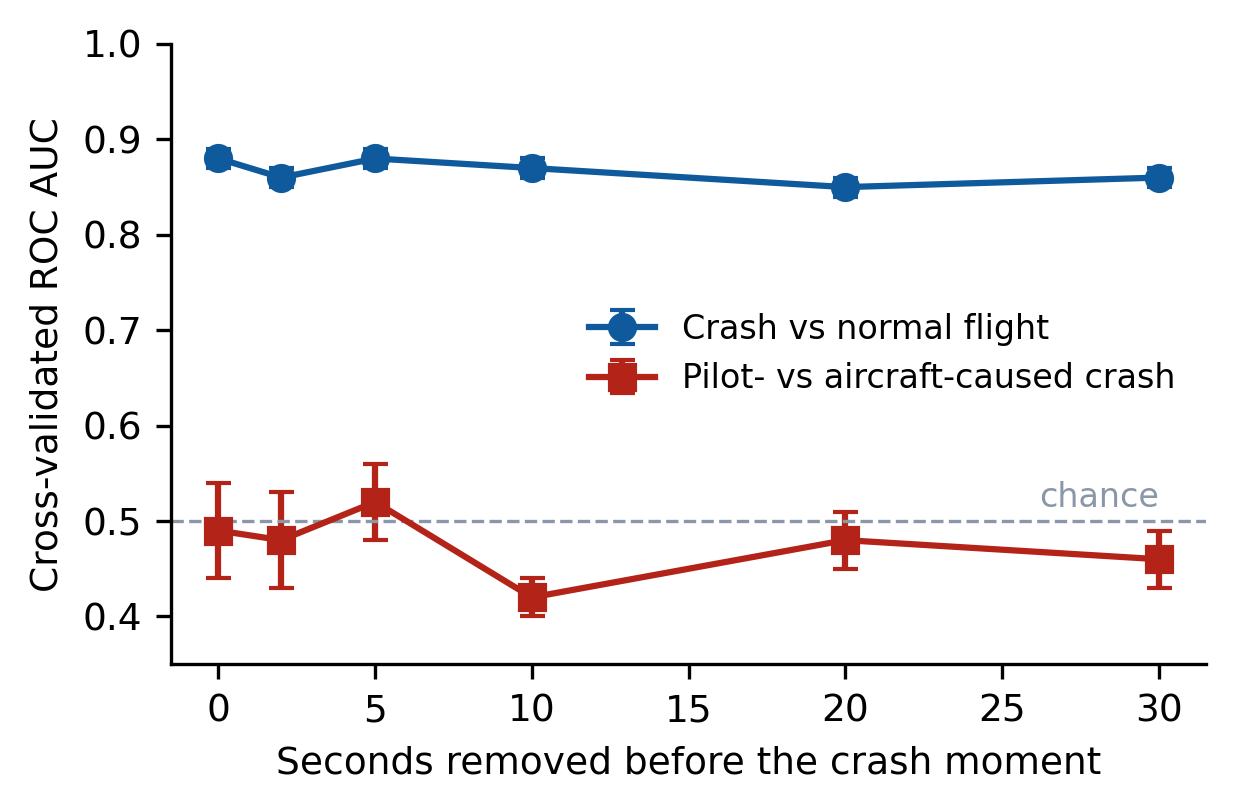
\includegraphics[width=0.72\textwidth]{fig_leak_curve.png}
\caption{Cross-validated AUC on the constant subset ($n=213$ for crash vs.\ normal, $n=89$ for pilot vs.\ aircraft) as the end of the analysis window moves away from the crash moment. Bars: 95\% bootstrap confidence intervals.}
\label{fig:leak}
\end{figure}

\subsection{Within the same drone and between drones (Q3b, Q3c)}
\label{sec:vibration}
Relative to the same drone's earlier flights, the crash flight was neither more vibrating ($\bar r=0.48$, 95\% CI
0.38--0.58, $p=0.67$, 61 drones) nor worse at tracking its commands ($\bar r=0.50$, 0.38--0.63, $p=0.47$, 46 drones;
Fig.~\ref{fig:within}). Presented as an exclusion bound, the upper 95\% confidence bound of 0.58 indicates absence of substantial pre-crash
vibration surges within the same drone of the magnitude observed between drones ($\bar r=0.67$). Relative to matched
drones without a recorded crash, drones that later crashed vibrated more on their ordinary pre-crash flights ($\bar r=0.67$,
0.57--0.77, $p=0.0023$, 60 sets; Holm-adjusted $p=0.016$), while the tracking error did not differ significantly
($\bar r=0.57$, 0.44--0.70, $p=0.15$, 47 sets). The vibration difference was clearest for aircraft-caused crashes
($\bar r=0.67$, $p=0.005$, 46 sets) and similar in size but not significant for pilot-caused ones ($\bar r=0.64$, $p=0.16$,
14 sets).

As a screening signal, the crashed drone was the roughest of its matched set in 33 of 60 sets (55.0\%, Wilson 95\% CI
42.5--66.9\%, against 40.3\% expected under the exact Poisson-binomial null; exact one-sided Poisson-binomial $p=0.0137$).
Furthermore, in 38 of 60 sets (63.3\%, Wilson 95\% CI 50.7--74.4\%), the crashed drone exceeded the third quartile (Q3) of
its matched controls. Sensitivity differed between measurement sources: 32 of 48 crashed drones (66.7\%, Wilson 95\% CI
52.5--78.3\%) exceeded control Q3 on the older estimator metric, compared to 6 of 12 (50.0\%, Wilson 95\% CI 25.4--74.6\%)
on the newer accelerometer metric.

In practical fleet operations, positive predictive value (PPV) depends heavily on the operational flag rate and the fleet base rate.
In the archive, 284 distinct vehicles accounted for all 520 real-hardware crash-rated logs out of 38,320 distinct vehicle identifiers,
establishing an empirical vehicle crash base rate of 0.741\% (284/38,320). When restricted to screenable multi-flight vehicles
(airframes with $\ge 2$ recorded flights, the operational prerequisite for pre-crash longitudinal screening), the crash base rate
is 0.689\% (182 crashed vehicles out of 26,421 multi-flight airframes). We emphasize that these base rates represent the lifetime probability
of an airframe ever receiving a crash rating in the archive index, rather than an operational flight-hour incident rate, because the public
archive does not record flight hours per airframe. Reported confidence intervals for PPV reflect sampling uncertainty in sensitivity
(derived via 10,000 bootstrap resamples over crashed cases); the operational base rate is treated as a fixed fleet parameter.
We evaluate screening performance under two distinct operational paradigms:

\emph{Empirical matched-set screening (45.1\% flag rate):} In our matched sets, flagging drones that exceed the upper quartile
of their matched controls yields 63.3\% sensitivity (38 of 60). Because sets contain 1 or 2 controls, the weighted null flag rate
is 45.1\%. At the 0.741\% vehicle base rate, this yields an operational PPV of 1.04\% (95\% bootstrap CI 0.83--1.25\%), an unflagged
risk of 0.496\%, a relative risk of $2.09\times$ over unflagged airframes, a lift of $1.40\times$ over base rate, and 96.4 inspections
per detected crash (PPV 0.96\%, 104 inspections per crash at the 0.689\% screenable base rate).

\emph{Fleet-wide reference screening:} Rather than comparing solely within small local sets, an operator can screen airframes against an
established reference distribution of non-crash control drones sharing the same flight controller hardware, firmware generation, and
measurement source (20 strata, 107 unique control drones filling 124 control slots, with 17 controls serving in more than one matched set;
overall AUC / mean percentile 0.689, 95\% CI 0.619--0.758). Each airframe is ranked against control flights within its matching hardware and sensor stratum.
Using Bayes' rule $\text{PPV} = \text{Sensitivity} \times \pi / \text{FlagRate}$, where the denominator $\text{FlagRate} = \text{Sensitivity} \times \pi + \text{FPR} \times (1 - \pi)$ is the population proportion flagged, screening at a 25\% flag rate identifies 50.0\% of crashed airframes (30 of 60, 95\% CI 36.7--63.3\%), yielding an
operational PPV of 1.48\% (95\% CI 1.09--1.88\%), an unflagged risk of 0.493\%, a relative risk of $3.00\times$, a lift of $2.00\times$
over the 0.741\% base rate, and 67.5 inspections per detected crash (at the 0.689\% screenable base rate: PPV 1.37\%, 95\% CI 1.01--1.74\%,
lift $1.99\times$, 73.1 inspections per crash).
Tightening the threshold to the top decile (10\% flag rate) achieves 33.3\% sensitivity (20 of 60, 95\% CI 21.7--45.0\%), an operational
PPV of 2.26--2.43\% (exact Bayes; 2.26\% at 0.689\% screenable base rate and 2.43\% at 0.741\% fleet base rate; nominal formula $\text{Sens} \times \pi / 0.10$ yields 2.30--2.47\%), with an unflagged risk of 0.510--0.549\%, a relative risk of $4.42--4.50\times$, a lift of $3.3\times$, and 41.2--44.2 inspections per detected crash.
Tightening further to the top 5\% (5.0\% flag rate) achieves 20.0\% sensitivity (12 of 60, 95\% CI 10.8--31.9\%), yielding an exact Bayes PPV of 2.90\% (95\% CI 1.57--4.63\%; nominal formula $\text{Sens} \times \pi / 0.05$ yields 2.96\%), a lift of $3.91\times$ over base rate, and 34.5 inspections per detected crash (nominal 33.7). Across all operating points, achieving a PPV $\ge 10\%$ ($\le 10$ inspections per true positive) at the 0.741\% base rate requires sensitivity $\ge 74.4\%$ at a 5\% false-alarm rate, which the observed ROC does not reach under the empirical vibration ROC curve (AUC 0.689).
Under a broader source-matched reference (matching on measurement source alone; AUC 0.655, 95\% CI 0.591--0.716), a 25\% flag rate yields
40.0\% sensitivity, PPV 1.19\% (lift $1.60\times$, 84.3 inspections per crash), rising to 25.0\% sensitivity, PPV 1.85\% (lift $2.50\times$,
54.0 inspections per crash) at the 10\% flag rate. We emphasize that because the 107 reference controls (filling 124 slots across 20 strata with 17 controls reused across sets) were drawn from the same archive pool as the matched sets, and because the exact Bayes PPVs assume an operational 10\% flag rate among non-crash drones rather than measuring realized flag rates across the entire 38,320-vehicle population, these PPV figures (2.26--2.43\%) represent an exploratory illustration conditional on the assumed flag rate and discovery sensitivity (20 of 60) rather than an independently frozen population benchmark. In all scenarios, vibration screening functions as a broad maintenance inspection filter rather than an operational crash warning.

\begin{figure}[t]
\centering
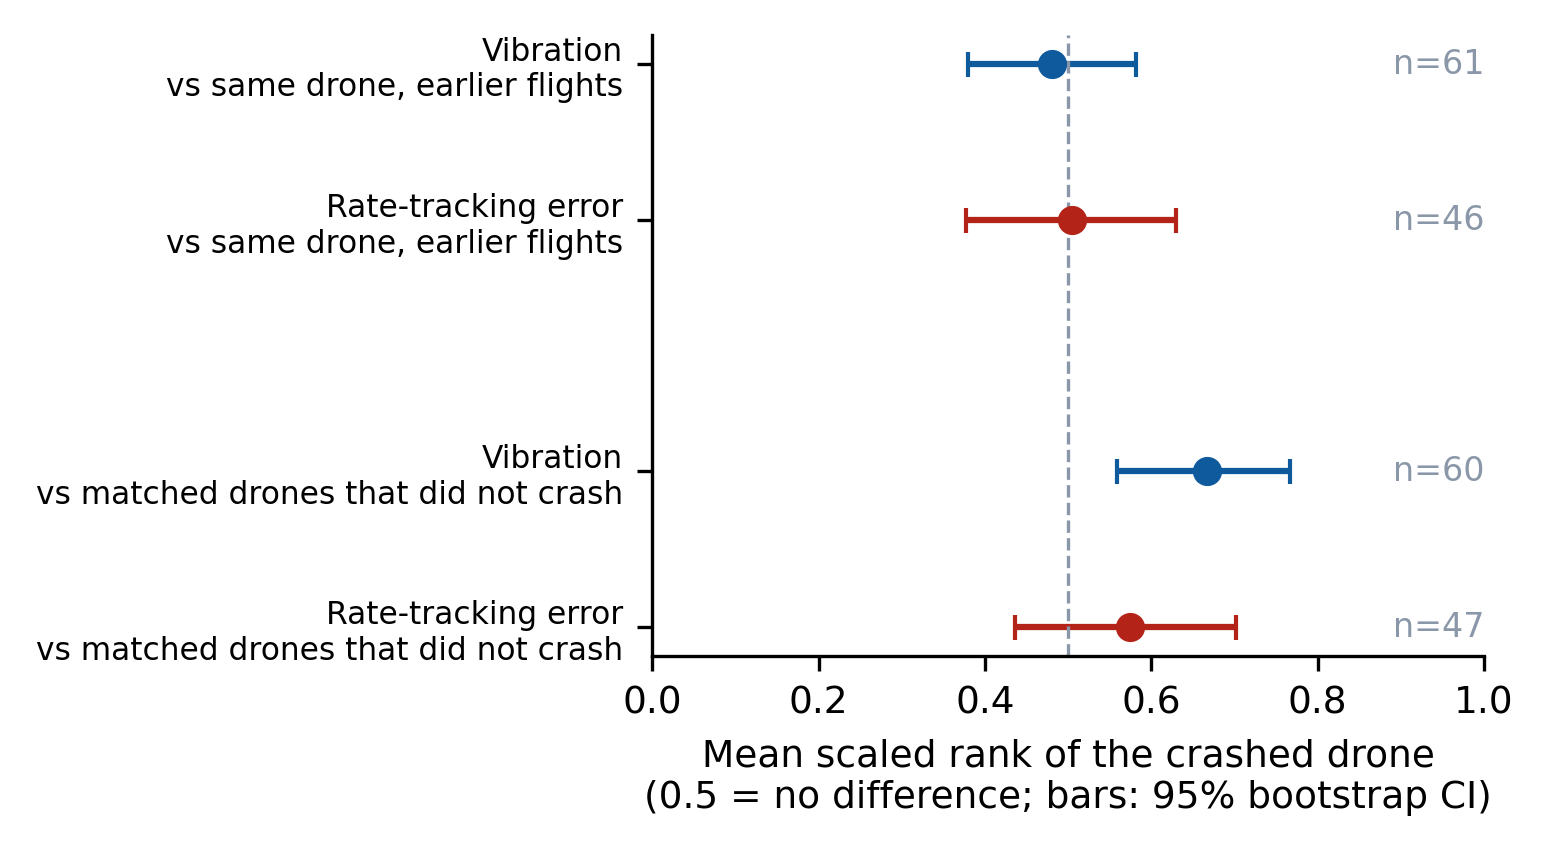
\includegraphics[width=0.78\textwidth]{fig_within_between.png}
\caption{Mean scaled rank of the crashed drone against its own earlier flights (top) and against matched drones
without a recorded crash (bottom). 0.5 indicates no difference.}
\label{fig:within}
\end{figure}

\subsection{Robustness of the between-drone result (exploratory)}
\label{sec:robust}
The vibration result held when controls were restricted to the same airframe as the case ($\bar r=0.69$, $p=0.008$,
39 sets), when case flights from the crash day were removed ($\bar r=0.76$, $p=0.003$, 25 sets) and after adjusting
for flight duration ($\bar r=0.69$, $p=0.0005$, 57 sets; Fig.~\ref{fig:robust}). Duration was barely correlated with
vibration (Spearman $\rho=0.05$ and $-0.04$ for the two measurement sources), although case flights were longer than
control flights (median 289\,s against 173\,s). The sharp sample shrinkage when removing crash-day flights (from 60 to 25
sets) indicates that many pre-crash flights in the public archive occurred during the same flight session or day. The archive
index did not record intra-day flight sequence. Across all 44 matched sets with exposure flights on the same calendar day as the crash, parsing raw GPS epoch timestamps confirmed that every pre-crash exposure flight strictly preceded the crash moment in time (0 post-crash flights occurred in the exposure window). This temporal ordering rules out post-accident flight inclusion, but points to potential confounding by development or tuning sessions
rather than progressive operational degradation: the ``maintenance view'' (vibration reflecting mechanical wear over time)
competes directly with an ``experimental airframe'' view (poorly tuned or prototype drones vibrate more and crash during
testing). Furthermore, matching was limited to flight controller hardware, PX4 major.minor version and vehicle type; it did
not control for propellers, payload, airframe size, or operator identity. To test whether the 17 controls reused across the 20 strata artificially inflated significance, we re-evaluated the test via a two-stage cluster bootstrap resampling both case airframes ($n=40$) and unique control airframes ($n=94$) across 2,000 resamples: the mean scaled rank was 0.662 with a 95\% cluster bootstrap CI of [0.536, 0.789] (control-only clustering yielded [0.587, 0.744]), both of which strictly exclude chance (0.50).

The vibration difference was carried by the older estimator metric ($\bar r=0.68$, $p=0.005$, 48 sets); within the original
cohort, the exploratory subset with the newer accelerometer metric showed a smaller, non-significant difference ($\bar r=0.62$,
$p=0.191$, 12 sets; Fig.~\ref{fig:robust}). A declared replication protocol on newer accelerometer logs selected 26 sets, yielding
19 usable matched sets ($9$ sets pooled from the initial cohort and $10$ new cases entirely outside the original test). On the 10 new
cases, the mean scaled rank was $\bar r=0.50$ (95\% CI 0.20--0.75, $p=0.5760$), which is inconclusive given the wide confidence interval.
Pooling all 19 usable sets gives $\bar r=0.58$ (95\% CI 0.39--0.76, one-sided $p=0.251$). A two-sample permutation test (100,000 draws) between the older estimator sets ($n=48$, mean scaled rank 0.677) and newer accelerometer sets ($n=19$, mean scaled rank 0.580) indicates that the difference in effect size is not statistically significant ($\Delta \bar r = 0.097$, two-sided permutation $p = 0.3221$), consistent with small-sample variability rather than structural divergence, though this heterogeneity test is underpowered given the sample sizes ($n=19$ vs.\ $48$). Statistical design power at $N=19$ for an
assumed effect of $\bar r=0.67$ was 0.379 (and 0.118 if the true effect
is $\bar r=0.58$). Statistical sample sizing at one-sided $\alpha=0.025$ indicates that detecting $\bar r=0.67$ ($\Delta=0.17$) with 80\%
power requires 55 matched sets; however, this assumes the discovery effect size was not inflated by winner's curse. If the true effect
size is closer to the pooled estimate of $\bar r=0.58$ ($\Delta=0.08$), 247 sets are required. Because 247 matched sets exceed the
capacity of the current single archive, resolving this effect definitively requires prospective multi-fleet partner deployments.

\begin{figure}[t]
\centering
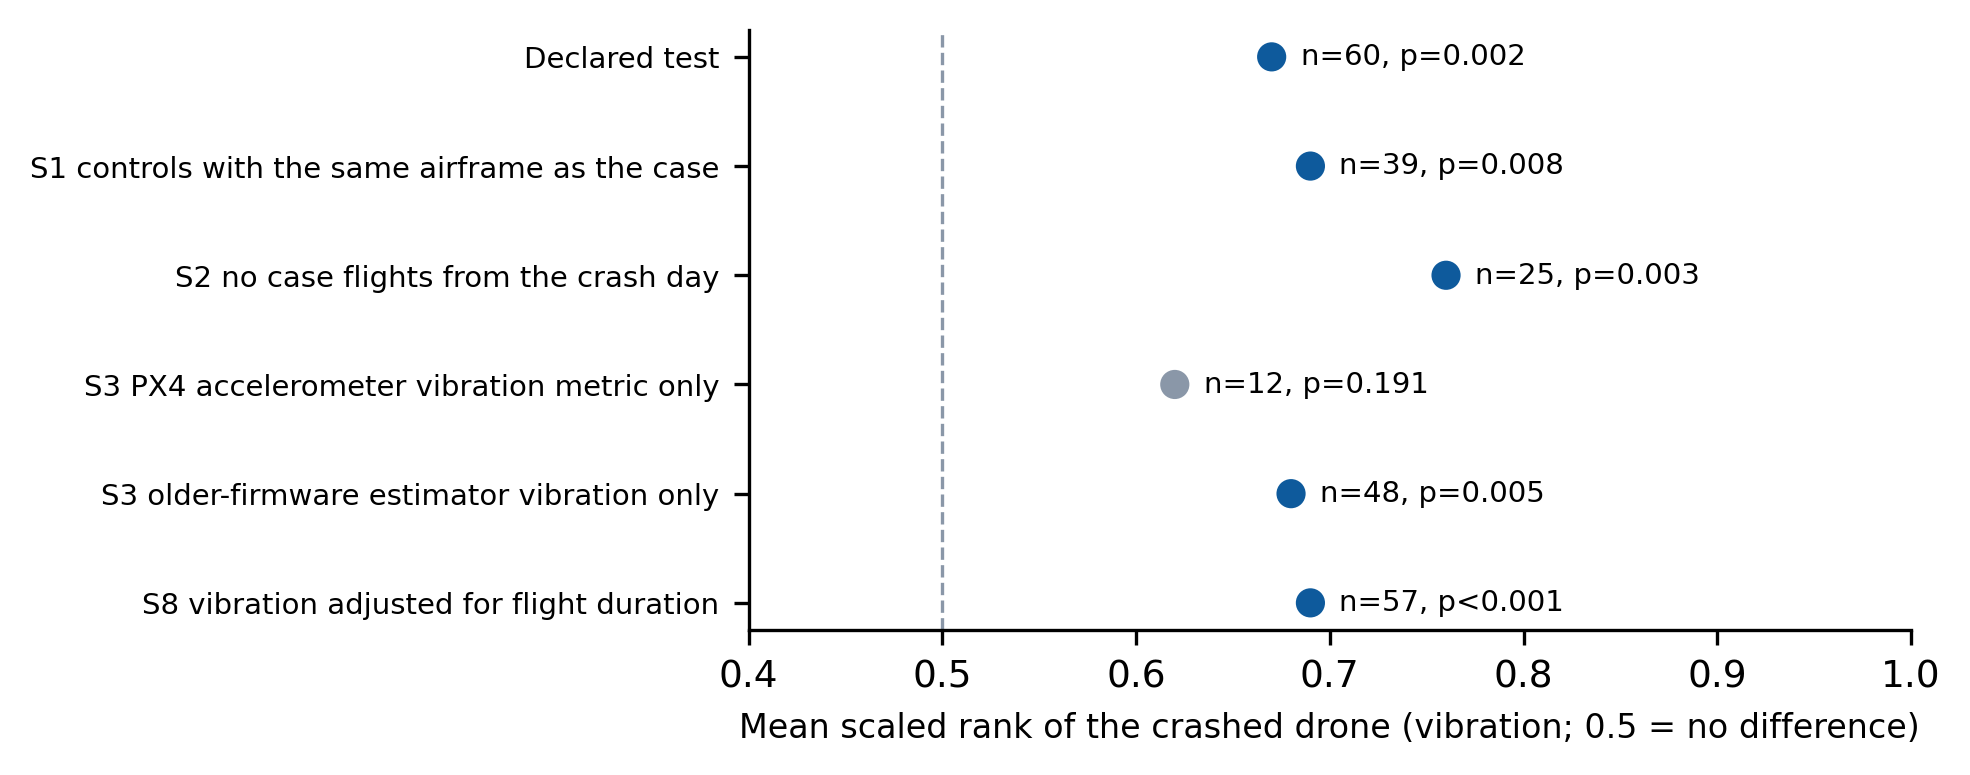
\includegraphics[width=0.78\textwidth]{fig_robustness.png}
\caption{Between-drone vibration result under alternative specifications (exploratory). Specification labels: S1: airframe-matched controls; S2: excluding case flights from the crash day; S3: stratification by vibration measurement source (older-firmware estimator metric vs.\ newer accelerometer metric); S8: log-linear adjustment for flight duration. Blue: $p<0.025$.}
\label{fig:robust}
\end{figure}

\subsection{Expert diagnoses (Q4)}
\label{sec:experts}
Of 148 forum threads describing a real crash, the expert attributed it to the aircraft in 94 (64\%), to the pilot in 9
(6\%), to both in 2, and was unclear or gave no diagnosis in 43 (29\%). Tuning or configuration was the cause named
most often (26 of 94; 14 of the 47 confirmed by the poster), followed by GPS, compass or estimator problems (18) and
motors, ESCs or propellers (16) (Fig.~\ref{fig:causes}). Of 14 threads whose log carried an aircraft crash rating in the index, the
expert agreed in 11 and was unclear in 3; none attributed the crash to the pilot. Download attempts across all 148 threads
yielded 43 downloadable logs from 43 distinct threads (38 aircraft-fault and 5 pilot-fault; the remaining 105 had unhosted
or expired external links). Of the 38 aircraft logs, exactly 35 were associated with checkable fault categories in
Table~\ref{tab:checks} (12 tuning, 5 vibration, 5 GPS, 9 motor, 4 battery).

Table~\ref{tab:checks} compares the fault checks with the full flight window ($m=0$\,s) and with the last 10\,s before
the crash removed ($m=10$\,s). With the window ending 10\,s before the crash, no check met the declared criterion.
The tuning check illustrates the diagnostic leakage described in Section~\ref{sec:window}: across all candidate logs with the full
window, the check fired on 10 of 12 (83.3\%). Across the 9 constant tuning logs with duration $\ge 10$\,s surviving the 10\,s
cut-off without sample attrition, firing dropped from 7 of 9 (77.8\%) with the full window to 1 of 9 (11.1\%) at $m=10$\,s
(6 logs lost firing, 0 gained; exact two-sided McNemar $p=0.03125$). However, normal-flight firing also fell from 18/142 (13\%)
to 7/130 (5\%), indicating that window shortening itself reduces cumulative exposure to threshold triggers alongside any crash-impact
leakage. Furthermore, this exploratory finding is descriptive rather than confirmatory: across the five diagnostic checks evaluated,
an unadjusted $p=0.031$ does not survive Bonferroni multiplicity correction ($p \approx 0.16$), and the other four checks exhibited
low baseline sensitivity even on full windows ($\le 25\%$, with 0/4 for motor and 0/2 for battery on paired logs), while tuning exceeded
the declared 10\% normal-flight false-alarm ceiling (13\%). Thus, while rate-tracking error demonstrated marked leakage, claims that
leakage is strictly confined to tuning must be tempered by the limited baseline sensitivity of the remaining checks.

To test diagnostic attribution on independently evaluated incidents, we evaluated the rule across all 43 downloadable logs behind
expert forum threads (38 aircraft-fault and 5 pilot-fault). As noted in Section~\ref{sec:data}, cross-tabulating these 43 logs against
archive ratings revealed that all 9 logs carrying an uploader rating were labeled \texttt{crash\_sw\_hw} (and all 9 were diagnosed as aircraft
faults by experts, 100\% agreement); the 5 expert pilot crashes were submitted unrated, which is consistent with, but not statistical
evidence of, reluctance to self-identify pilot fault: all 5 pilot logs were unrated in the index against 28 of 38 aircraft logs unrated
(one-sided Fisher exact $p=0.25$). Evaluated on the 38 aircraft incidents, the fixed rule predicted ``aircraft'' in 18 (47.4\%),
``unknown'' in 6 (15.8\%), and erroneously blamed the ``pilot'' in 14 (36.8\%). On decided aircraft cases ($n=32$), the rule was wrong on
43.8\% (14/32). Detailed inspection of flight mode sequences confirmed the failure mechanism: in all 14 misclassified logs, the vehicle was
in a pilot-flown mode at the crash moment (\texttt{POSCTL} in 7 logs, \texttt{STAB} in 4, \texttt{ALTCTL} in 3; including log \texttt{e9034973},
which transitioned \texttt{POSCTL} $\to$ \texttt{AUTO\_4} $\to$ \texttt{POSCTL} as the pilot attempted manual recovery). Because no hardware
failsafe fired before impact, the rule defaulted to blaming the pilot.

Conversely, when evaluated on the 5 pilot-fault incidents, the fixed rule predicted ``aircraft'' in 4 (80.0\%) and ``pilot'' in only 1 (20.0\%;
pilot recall 1 of 5, exact Clopper--Pearson 95\% CI 0.5--71.6\%, Wilson 3.6--62.4\%), misclassifying 4 of 5 pilot crashes because motor saturation,
accelerometer clipping, or failsafe activation occurred as the vehicle struck the ground. Combining both classes across all 37 decided expert logs
(32 aircraft, 5 pilot), the rule produced 18 incorrect decisions out of 37 (48.6\% error rate), yielding a balanced accuracy of
$(56.25\% + 20.0\%) / 2 = 38.1\%$ (Bayesian 95\% credible interval 0.25--0.61 from independent Jeffreys beta posteriors; conservative class-averaged Clopper--Pearson bounds 0.19--0.73, formed as the unweighted mean of the separate exact binomial 95\% confidence intervals for aircraft recall [18/32: 37.6--74.3\%] and pilot recall [1/5: 0.5--71.6\%]). Because this wide interval contains both chance (0.50) and the declared pass mark (0.70), this independent evaluation is statistically inconclusive and cannot exclude agreement at the declared pass mark. When evaluated on the subset of 34 logs with complete telemetry required by the statistical models (30 aircraft, 4 pilot), the rule decided 29 cases (25 aircraft, 4 pilot), predicting aircraft in 15 of 25 aircraft and 4 of 4 pilot, yielding a balanced accuracy of $(60.0\% + 0.0\%) / 2 = 30.0\%$. Of the 30 complete aircraft logs, exactly 5 overlapped with the 148 modelled crashes in the training pool (all 5 rated \texttt{crash\_sw\_hw} in the index; 0 pilot logs overlapped). Evaluating the cross-validated logistic regression model across all 34 complete logs yielded predictions of ``aircraft'' in 27 of 30 aircraft logs (90.0\%) and in all 4 pilot logs (0/4 pilot recall; covering 4 of the 5 pilot logs because one lacked actuator or setpoint topics), defaulting strongly toward its aircraft training prior (75.7\% prevalence; 112/148) for a balanced accuracy of $(90.0\% + 0.0\%) / 2 = 45.0\%$ and ROC AUC of $0.467$ (95\% bootstrap CI 0.211--0.733). When the 5 overlapping logs were excluded ($n=29$: 25 aircraft, 4 pilot), the logistic regression model achieved AUC 0.450 (95\% bootstrap CI 0.185--0.715); given the wide confidence interval spanning from 0.185 to 0.715 on 29 logs, this evaluation provides no evidence of discrimination and remains inconclusive. Across both heuristic rules and statistical models on this sample, log-based telemetry attribution showed no discriminative agreement above chance. We emphasize the caveat
that this evaluation measures agreement between heuristic rules or models and expert community reading of the same telemetry, rather than ground truth:
original posters explicitly confirmed the diagnosis in only 47 of 94 aircraft-fault threads (50.0\%) and 5 of 9 pilot-fault threads (55.6\%).
Nonetheless, this independent evaluation illustrates the challenge of log-based attribution: neither the heuristic rule nor the statistical model demonstrated reliable agreement above chance.

\begin{table}[t]
\centering
\caption{Fault checks on logs whose expert named the matching fault, with the full window ($m=0$\,s) and with the last 10\,s
before the crash removed ($m=10$\,s). Declared criterion: at least 50\% of diagnosed logs and at most 10\% of normal flights.
Paired columns show constant logs surviving across both windows.}
\label{tab:checks}
\footnotesize
\setlength{\tabcolsep}{2.5pt}
\begin{tabularx}{\textwidth}{@{}Xcccccc@{}}
\toprule
 & \multicolumn{2}{c}{Diagnosed ($m=0$\,s)} & Diagnosed & Paired $\Delta$ & \multicolumn{2}{c}{Normal comparison} \\
\cmidrule(lr){2-3} \cmidrule(lr){4-4} \cmidrule(lr){5-5} \cmidrule(lr){6-7}
Expert-named fault & All logs & Paired & $m=10$\,s & ($p$-value) & $m=0$\,s & $m=10$\,s \\
\midrule
Tuning or configuration & 10/12 (83\%) & 7/9 (78\%) & 1/9 (11\%) & $-6$ ($p=0.031$) & 18/142 (13\%) & 7/130 (5\%) \\
Vibration or mounting & 3/5 (60\%) & 3/5 (60\%) & 3/5 (60\%) & 0 ($p=1.00$) & 7/48 (15\%) & 4/38 (11\%) \\
GPS, compass or estimator & 1/5 (20\%) & 1/4 (25\%) & 1/4 (25\%) & 0 ($p=1.00$) & 10/143 (7\%) & 5/130 (4\%) \\
Motor, ESC or propeller & 1/9 (11\%) & 0/4 & 0/4 & 0 ($p=1.00$) & 8/143 (6\%) & 5/130 (4\%) \\
Battery or power & 0/4 & 0/2 & 0/2 & 0 ($p=1.00$) & 4/143 (3\%) & 1/130 (1\%) \\
\bottomrule
\end{tabularx}
\end{table}

\begin{figure}[t]
\centering
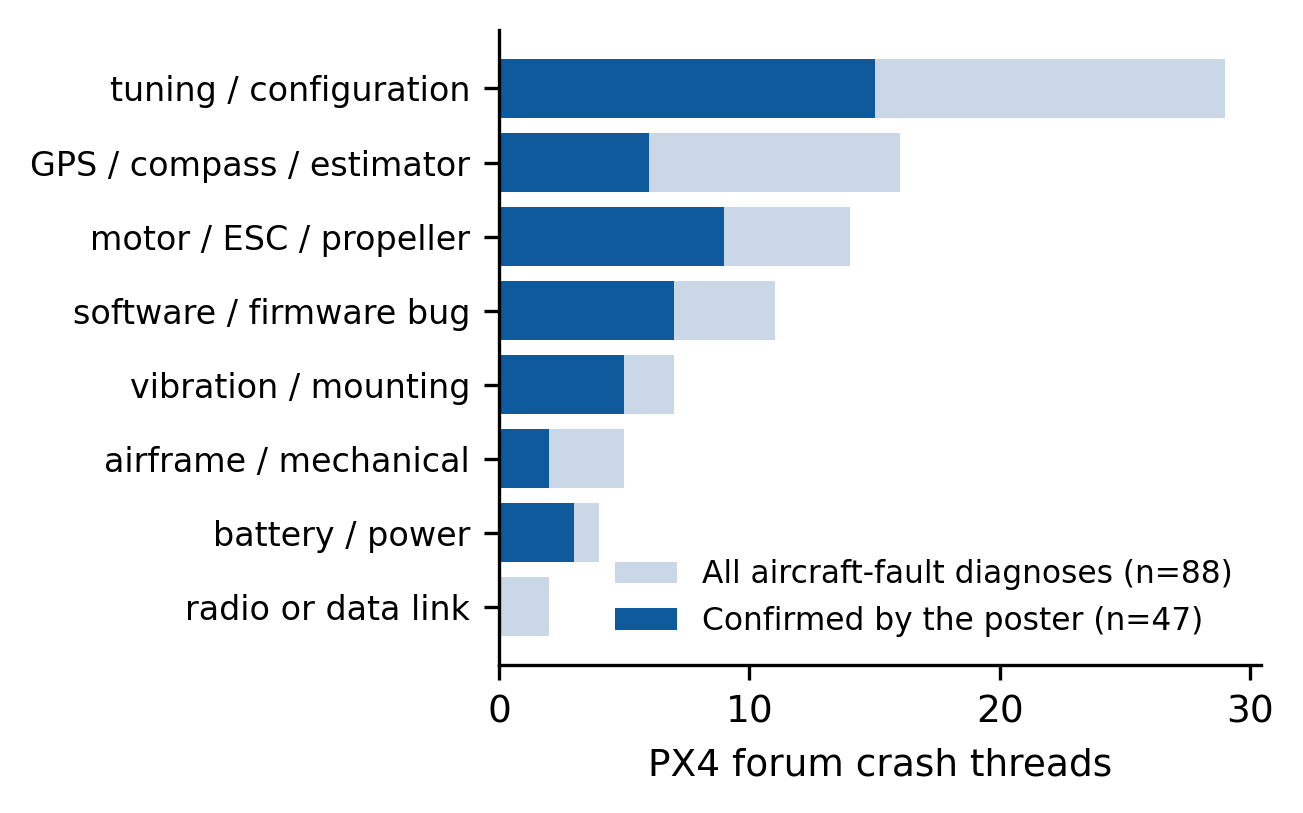
\includegraphics[width=0.78\textwidth]{fig_forum_causes.png}
\caption{Causes named by experts in PX4 forum threads that attributed a crash to the aircraft.}
\label{fig:causes}
\end{figure}

\subsection{Exploratory evaluation of language-model review panels (preliminary)}
\label{sec:lm_summary}
Because language-model assistants are increasingly proposed for automated flight log analysis, we conducted a preliminary exploratory evaluation on 60 author-generated fault cases using four local models (3--4B parameters) configured both as single agents and as multi-agent review panels (Table~\ref{tab:llm}). While a fixed deterministic rule achieved 75\% accuracy (naming the true cause in 35 of 50 active cases and correctly abstaining on 10 no-cause cases) with 0\% error (referring 15 cases to human operators), local language models produced substantial error rates (10--63\% wrong), suffered from mode collapse or complete abstention on active causes, and proved highly vulnerable to consensus manipulation: in a worst-case sensitivity sweep, a single compromised reviewer systematically flipped the panel's consensus decision in 45 to 56 of the 60 cases. In contrast, deterministic numeric telemetry extraction into code prevented direct prompt injection by construction across 40 hostile input strings. This exploratory comparison indicates that the tested small local models and review-panel configurations were unreliable on the 60 author-generated cases. Because the cases and fixed rule were developed by the same authors, the comparison is not an independent benchmark and should not be generalized to language models as a class or larger architectures. These preliminary results emphasize that multi-agent consensus voting without cryptographic proofs or fact-citation constraints cannot provide dependable safety assurance.

\begin{table}[!htbp]
\centering
\caption{Language-model review panels on 60 generated cases: counts of right (R), wrong (W), and deferred (Def) cases, with coverage (Cov., share of cases decided) and accuracy when answering (Acc.). ``Right'' includes correctly leaving a no-cause case open. Single-agent gemma3 and phi4 answered only the 10 no-cause cases (0\% coverage on active causes). Adversary flips show consensus changes caused by a single compromised reviewer in a worst-case sweep.}
\label{tab:llm}
\footnotesize
\setlength{\tabcolsep}{2.5pt}
\begin{tabular*}{\textwidth}{@{\extracolsep{\fill}}l ccc ccc c@{}}
\toprule
& \multicolumn{3}{c}{Single agent} & \multicolumn{3}{c}{Review panel} & Compromised \\
\cmidrule(lr){2-4} \cmidrule(lr){5-7}
Method & R / W / Def & Cov. & Acc. & R / W / Def & Cov. & Acc. & Flips / 60 \\
\midrule
Fixed rule (no model) & 45 / 0 / 15 & 75\% & 100\% & -- & -- & -- & -- \\
\texttt{gemma3:4b} & 10 / 0 / 50 & 17\%$^\dagger$ & 100\%$^\dagger$ & 3 / 36 / 21 & 65\% & 7.7\% & 49 \\
\texttt{phi4-mini} & 10 / 0 / 50 & 17\%$^\dagger$ & 100\%$^\dagger$ & 20 / 19 / 21 & 65\% & 51.3\% & 56 \\
\texttt{qwen2.5:3b} & 9 / 44 / 7 & 88\% & 17.0\% & 10 / 6 / 44 & 27\% & 62.5\% & 54 \\
\texttt{qwen3:4b} & 0 / 41 / 19 & 68\% & 0.0\% & 17 / 38 / 5 & 92\% & 30.9\% & 45 \\
\bottomrule
\end{tabular*}
\vspace{2pt}
{\footnotesize $^\dagger$Answered only on the 10 no-cause cases where abstention coincided with the ground truth; 0\% coverage on active causes.\par}
\end{table}

\subsection{Analyses added during revision (exploratory)}
\label{sec:posthoc}
To preserve the boundary between pre-declared confirmatory hypotheses (committed to version control on 20--24 October 2026; Table~\ref{tab:registration}) and exploratory investigations added during revision \cite{nosek2018prereg}, Table~\ref{tab:posthoc} documents each analysis added during peer review, its motivation, key results, git commit hash, first archive date in Software Heritage, and analysis run date. Exploratory analyses added during review are marked with $^\dagger$ throughout the text and tables. None of these exploratory additions altered the conclusions of the pre-declared tests; rather, they established empirical bounds on between-airframe confounding, tested alternative architectures, and quantified operational fleet screening performance.

\begin{table}[t]
\centering
\caption{Exploratory analyses added during peer review, their motivation, key results, git commit hashes, first archived dates in Software Heritage (\nolinkurl{swh:1:rev:bad06ff1256865c7e63d44389aac174e0281291d}, \nolinkurl{swh:1:rev:bbdd0420de4547ac7d67b84165292a46237b604d}, \nolinkurl{swh:1:rev:624dd694e0d207dd9c44b1c9550faaf04453bc56}, and \nolinkurl{swh:1:rev:3a9aa89417fa9ea2a2334e3a4794e2358fb713ee}), and analysis run dates.}
\label{tab:posthoc}
\scriptsize
\setlength{\tabcolsep}{2.0pt}
\begin{tabularx}{\textwidth}{@{}l X X c c c@{}}
\toprule
Analysis & Motivation & Key result & Commit & Archived & Run \\
\midrule
1,000-permutation null (Task B)$^\dagger$ & Calibrate detection threshold & Null mean 0.497; observed AUC upper bounds 0.510--0.619 (80\% power MDE 0.75) & \texttt{bad06ff} & 2026-10-25 & 2026-10-25 \\
Depth-1 decision stumps (Task B)$^\dagger$ & Test single-feature non-linear splits & Stumps AUC $0.430 \to 0.413$ at $m=10$\,s (upper bounds 0.534 and 0.528) & \texttt{bad06ff} & 2026-10-25 & 2026-10-25 \\
Constant-subset leak curve$^\dagger$ & Exclude sample attrition ($n=213$) & AUC declines smoothly $0.895 \to 0.868$ ($m=10$\,s) & \texttt{bbdd042} & 2026-10-25 & 2026-10-25 \\
Paired diagnostic leakage test$^\dagger$ & Test leakage on constant logs ($n=9$) & Tuning check $7/9 \to 1/9$, exact McNemar $p=0.03125$ & \texttt{bbdd042} & 2026-10-25 & 2026-10-25 \\
Same-sample decomposition$^\dagger$ & Account for airframe \& duration confounds & Changing comparison from other aircraft to same aircraft lowers AUC 0.83--0.88 to 0.53--0.57; CV design makes no detectable difference & \texttt{eb463b5} & 2026-10-25 & 2026-10-25 \\
Poisson-binomial set null$^\dagger$ & Account for mixed set sizes ($n=60$) & Exact null rate 40.28\%; observed 55.0\% ($p=0.0137$) & \texttt{bad06ff} & 2026-10-25 & 2026-10-25 \\
Screening PPV and CIs$^\dagger$ & Quantify operational fleet value & Exploratory illustration: fleet PPV 2.26--2.43\% (exact Bayes) at assumed 10\% flag rate ($3.3\times$ lift) & \texttt{bad06ff} & 2026-10-25 & 2026-10-25 \\
Sensitivity by vibration source$^\dagger$ & Compare older vs.\ newer metrics & Older: 32/48 (66.7\%); newer: 6/12 (50.0\%); pooled newer $\bar r=0.58$ ($p=0.25$) & \texttt{624dd69} & 2026-10-25 & 2026-10-25 \\
Independent 43-log validation$^\dagger$ & Evaluate against independent causes & Balanced accuracy 38.1\% (conservative CP 0.19--0.73); pilot recall 1/5; inconclusive & \texttt{3a9aa89} & 2026-10-25 & 2026-10-25 \\
Cohort selection step 4b$^\dagger$ & Isolate comparison vs.\ cohort effect & 67 multi-flight crashes vs.\ other-aircraft controls: AUC 0.522 [0.413, 0.615] & \texttt{f152d07} & 2026-10-26 & 2026-10-26 \\
Within-drone duration caliper$^\dagger$ & Test duration confounding in cohort & Caliper $\le 0.25$ matching lifts within-drone AUC $+0.110$ (0.532 to 0.642) & \texttt{f152d07} & 2026-10-26 & 2026-10-26 \\
Depth-3 tree bounds across cuts$^\dagger$ & Bound non-linear model performance & Upper bounds 0.519--0.724; collapses to 0.524 under 10\,s leakage control & \texttt{dfbabaf} & 2026-10-26 & 2026-10-26 \\
Fixed-score permutation null$^\dagger$ & Test CV fold-splitting variance & Fixed score SD 0.055 matches asymptotic theory (0.056); 0.090 reflects refitting variance & \texttt{dfbabaf} & 2026-10-26 & 2026-10-26 \\
Control cluster adjustment$^\dagger$ & Test control reuse robustness & Mean rank 0.665, 95\% cluster CI [0.587, 0.744]; heterogeneity $p=0.322$ & \texttt{dfbabaf} & 2026-10-26 & 2026-10-26 \\
Single vs.\ multi-history crashes$^\dagger$ & Test maiden-flight artifact hypothesis & Single-history ($n=45$) AUC 0.835 vs.\ multi-history ($n=103$) 0.891 at $m=0$\,s; cross-sectional separation is archive-wide & \texttt{aa1d7c6} & 2026-10-26 & 2026-10-26 \\
Duration caliper gradient \& CI$^\dagger$ & Quantify caliper sensitivity & Lift curve $\epsilon \in [0.10, 1.00]$; paired cluster bootstrap 95\% CI for $\Delta=+0.125$ is [+0.074, +0.238] & \texttt{aa1d7c6} & 2026-10-26 & 2026-10-26 \\
Two-stage cluster bootstrap \& GPS$^\dagger$ & Audit same-day timing \& clustering & Two-stage cluster CI [0.536, 0.789] over case \& control clusters; 44 same-day sets confirmed 0 post-crash flights & \texttt{aa1d7c6} & 2026-10-26 & 2026-10-26 \\
Rule balanced accuracy across cuts$^\dagger$ & Audit attribution rule across margins & BA declines smoothly from 0.460 ($m=0$\,s) to 0.454 ($m=5$), 0.393 ($m=10$), 0.371 ($m=20$), 0.350 ($m=30$) & \texttt{aa1d7c6} & 2026-10-26 & 2026-10-26 \\
\bottomrule
\end{tabularx}
\end{table}

\FloatBarrier
% ===================================================================
\section{Design implications for fleet assurance}
\label{sec:tool}

To translate these empirical findings into operational practice, we developed AeroFleet~2.0 (\url{https://github.com/AdityaPathare46/aerofleet}), an open-source, ground-side assurance tool for PX4 and ArduPilot fleets. The tool reads existing flight logs and configuration files without executing unverified autonomous decisions or contacting the aircraft in flight. Table~\ref{tab:design} maps each empirical finding from Sections~\ref{sec:data}--\ref{sec:results} directly to an assurance design implication.

In accordance with our negative attribution results (Q1--Q2), the tool presents a structured, chronological event review reporting evidence quality (dilution of precision, sensor health, and mode transitions) while strictly abstaining from issuing automated pilot-versus-aircraft liability verdicts. Responding to the vibration finding (Q3), the tool ranks airframes longitudinally against comparable peers within the same fleet to prioritize the top decile (10\%) for physical maintenance inspection (exploratory illustration: PPV 2.26--2.43\% [exact Bayes], lift $3.3\times$ at an assumed 10\% flag rate, 41--44 inspections per crash), rather than issuing per-flight crash alarms. Finally, to ensure evidentiary integrity over the lifecycle of each airframe, all reviews, approvals, and configuration checks are appended to a tamper-evident, Ed25519-signed record referencing SHA-256 digests of the original telemetry files.

\begin{table}[!htbp]
\centering
\caption{From empirical findings to design implications in fleet assurance.}
\label{tab:design}
\small
\begin{tabularx}{\textwidth}{@{}l X X@{}}
\toprule
Finding & Empirical result (Section) & Design implication for fleet assurance \\
\midrule
Attribution failure & Across the telemetry features, rules, and models evaluated here, logs do not separate pilot from aircraft causes above chance (balanced accuracy 0.47 on held-out test, 0.381 on expert set, 95\% CrI 0.25--0.61; §\ref{sec:attribution}, §\ref{sec:experts}) & Present time-ordered event chronology and data quality metrics; abstain from automated fault verdicts. \\
Diagnostic leakage & Apparent diagnostic check accuracy is consistent with crash-window leakage (tuning check sensitivity falls $7/9 \to 1/9$, exploratory; §\ref{sec:window}, §\ref{sec:experts}) & Remove crash impact window ($m \ge 10$\,s) and compare against aircraft operating baseline before diagnosing faults. \\
Between-drone vibration & Retrospective between-airframe association on older estimator metrics (mean rank 0.67, Holm $p=0.016$; provisional screening signal; §\ref{sec:vibration}) & Rank drones longitudinally against fleet peers; prioritize top decile (10\%) for mechanical maintenance inspection. \\
Confounding shrinkage & Changing comparison from other aircraft to same aircraft lowers AUC from 0.88 to 0.53--0.57 (§\ref{sec:confounding}) & Evaluate airframe health against its own flight history, not cross-sectional fleet averages. \\
Audit integrity & Multi-agent consensus voting is vulnerable to reviewer manipulation in exploratory 60-case setup (§\ref{sec:lm_summary}) & Rely on deterministic numeric telemetry extraction and append reviews to a tamper-evident, signed log. \\
\bottomrule
\end{tabularx}
\end{table}

\subsection{Recommended reporting checklist for flight-log diagnostics}
\label{sec:checklist}
To support drone safety regulators, accident investigators, and data-driven diagnostic tool developers in avoiding the leakage and confounding traps quantified in this study, Table~\ref{tab:checklist} outlines an eight-item recommended reporting checklist. Each item pairs a methodological recommendation with its empirical rationale and the specific failure mode observed in our experiments when that control is omitted.

\begin{table}[!htbp]
\centering
\caption{Recommended checklist for leakage-controlled evaluation and reporting of UAV flight-log diagnostic models and accident analytics.}
\label{tab:checklist}
\small
\begin{tabularx}{\textwidth}{@{}l p{0.32\textwidth} X@{}}
\toprule
Checklist Item & Methodological Recommendation & Rationale and Empirical Failure Mode \\
\midrule
1. Event-window removal & Remove $\ge 10$\,s prior to physical impact or ground tumble ($m \ge 10$\,s) & Consistent with crash-window leakage in individual physical checks (tuning sensitivity fell $7/9 \to 1/9$, exploratory; clipping fell 37\%), though cross-sectional AUC was stable ($0.88 \to 0.87$, §\ref{sec:window}). \\
2. Airframe-grouped folds & Partition cross-validation folds strictly by vehicle UUID & Prevents cross-fold identity memorization; while vehicle grouping alone did not lower AUC in our disjoint-operator sample ($0.884$ vs $0.883$), literature and independent validation establish its necessity when airframes recur. \\
3. Longitudinal baseline & Evaluate cases against the airframe's own pre-incident flights & Disentangles airframe confounding, though in uncurated archives an uncalipered longitudinal baseline alone yielded no detectable precursor signal (AUC 0.569, cluster CI [0.500, 0.643]) without duration matching. \\
4. Duration caliper matching & Enforce duration matching ratio ($|\Delta \ln(\text{duration})| \le 0.25$ to $\le 0.50$) & Aborted/short incident flights induce spurious duration separation; caliper matching recovers $+0.110$ within-drone AUC (paired cluster CI [+0.074, +0.238]), reversing duration masking (§\ref{sec:confounding}). \\
5. Two-class expert ground truth & Validate against multi-coder independent diagnoses with reported agreement ($\kappa \ge 0.70$) & Uploader labels are noisy and biased; evaluation should quantify inter-rater reliability across both pilot-fault and aircraft-fault classes (§\ref{sec:experts}). \\
6. Operational base-rate calibration & Report exact Bayes PPV, relative risk, and inspections per event using fleet base rates & High ROC AUCs mask severe false-alarm fatigue in operational deployment under sparse event base rates ($\le 1\%$, §\ref{sec:vibration}). \\
7. Prospective protocol registration & Pre-specify hypotheses, sample funnels, features, models, seeds, and pass marks in version control & Eliminates $p$-hacking, outcome switching, and post-hoc rationalization of exploratory fluctuations (§\ref{sec:protocol}). \\
8. Persistent open artifact deposit & Deposit raw logs, extraction code, and derived feature tables in public archives & Ensures cryptographic provenance, auditability, and independent re-analysis across research groups. \\
\bottomrule
\end{tabularx}
\end{table}

% ===================================================================
\section{Discussion}
\label{sec:discussion}

\paragraph{Attribution} A declared rule, its held-out replication and cross-validated models all found no usable
separation between pilot- and aircraft-caused crashes with these labels and features. Because pilot labels are sparse
(only 36 pilot-labelled crashes in the modelling sample against 112 aircraft-labelled crashes), 80\% power requires an AUC of roughly 0.65 under asymptotic Wilcoxon theory (0.75 under
the empirical permutation null; permutation 97.5th percentile 0.660 has $\approx 50\%$ power); observed cross-validated
models yield empirical 95\% bootstrap upper bounds between 0.510 and 0.619. An operational attribution verdict would require
an AUC of approximately 0.8 or higher, which these models do not approach. Furthermore, independent evaluation against
43 expert forum cases was statistically inconclusive (balanced accuracy 0.381, Bayesian 95\% CrI 0.25--0.61 from independent
Jeffreys beta posteriors, class-averaged Clopper--Pearson bound 0.19--0.73; cannot exclude agreement at the declared 0.70 pass
mark; pilot recall 1 of 5, exact Clopper--Pearson 95\% CI 0.5--71.6\%; conservative class-averaged bound 0.19--0.73). Our prospectively declared negative result applies to linear models and decision stumps; exploratory depth-3 decision trees across cut-offs yielded AUCs of 0.366--0.603 (upper bounds 0.519--0.724), with the upper bound dropping to 0.524 at $m=10$\,s, confirming that non-linear trees also fall within chance under leakage control. Across the telemetry features, rules, models, and
validation procedures evaluated here, we found no reliable above-chance separation of pilot-caused and aircraft-caused
crashes. This result bounds the evidence available in the present dataset and setup; it does not establish that attribution
is impossible under all sensors, labels, models, or operating conditions.
While commercial and legal disputes often seek a binary verdict, aviation safety science demonstrates that accidents are
multi-causal systemic events involving organizational, environmental and human factors \cite{wiegmann2003hfacs}. Uploader
labels are noisy, and the divergence between uploader pilot blame (32\%) and expert forum diagnoses (6\%) may reflect
several untested mechanisms, including differing definitions of pilot responsibility among autopilot developers or
differing thresholds for public fault attribution. A log records the combined
physical outcome of pilot inputs, environmental disturbances and vehicle response; disentangling responsibility from telemetry
alone is not supported by the data. Tools that issue automatic responsibility verdicts should be evaluated against independent
investigations before adoption.

\paragraph{Leakage and confounding} While cross-sectional models on the discovery sample showed high apparent separation (AUC 0.88), our decomposition demonstrated that vehicle-grouped cross-validation (0.884) and crash-window removal (0.860) made no detectable difference. Crucially, isolating cohort selection from comparison population effects reveals that evaluating the exact same 67 multi-flight crashes against independent other-aircraft normal flights collapses model AUC to 0.522 [0.413, 0.615] (Step~4b). This indicates that the drop from 0.83--0.88 to 0.53--0.57 is primarily driven by cohort selection across evaluation samples (the multi-flight cohort lacks separable precursors cross-sectionally as well as longitudinally), rather than by within-drone baseline adjustment alone. On the identical 372 flights of the multi-flight cohort, cross-sectional evaluation (0.529 [0.453, 0.607]) and within-drone Group-CV (0.569 [0.493, 0.645]; cluster bootstrap 95\% CI [0.500, 0.643]; pairwise mean AUC 0.592 [0.516, 0.692]) yielded overlapping intervals (the cluster bootstrap interval touches chance at 0.500, while the pairwise interval extends down to near-chance at 0.516), indicating that uncalipered matching yields no detectable precursor signal in this cohort. However, controlling for feature-window duration within drones via caliper matching ($|\Delta \ln(\text{duration})| \le 0.25$) lifts within-drone AUC from 0.532 to 0.642 ($+0.110$ on the exact same 36 airframes; paired cluster bootstrap 95\% CI [+0.074, +0.238]), suggesting that baseline duration differences between crash and non-crash flights mask within-drone precursor detection in this cohort. Diagnostic checks were also \textit{consistent with} crash-window leakage: specifically, tuning fault detection
fell from 7/9 to 1/9 sensitivity (unadjusted $p=0.031$ on paired logs) when the final 10\,s were removed, accompanied by
a drop in normal-flight firing from 13\% to 5\% which suggests that shorter windows reduce trigger exposure alongside
leakage. Furthermore, this finding is exploratory, does not survive Bonferroni correction over five checks ($p \approx 0.16$),
and the low baseline sensitivity of the remaining checks ($\le 25\%$) leaves open whether other physical failure modes
exhibit the same pattern. In interpreting feature signals, two operational definitions of motor saturation must be distinguished: the whole-flight cumulative summary feature used in predictive models ($\texttt{sat\_frac}$, the fraction of armed flight time with any motor at $\ge 95\%$ authority), versus the discrete threshold check used in the attribution rule (motor output at $\ge 95\%$ authority for $\ge 1.0$\,s cumulative during the final 10\,s before $t_c$). Furthermore, while crash-flight analysis windows terminate at impact or tilt, normal-flight comparison windows end at disarm (encompassing the complete descent, flare, touchdown, and landing sequence), which contributes to duration differences and baseline feature exposure. Regardless of the precise mechanism, we recommend that diagnostic evaluations remove the crash window,
control for flight duration, and compare against an aircraft's own operating baseline before claiming pre-crash anticipation.

\paragraph{Drone-level risk} The positive result concerns airframes, not flights. Drones that later crashed vibrated
more than comparable drones on ordinary flights, consistent with a maintenance view in which mechanical degradation
precedes catastrophic failure \cite{petritoli2018reliability}. However, two important qualifications apply. First,
removing crash-day flights raised $\bar r$ from 0.67 to 0.76 ($p=0.0027$, 25 sets), which cuts against a same-session
flight disturbance explanation; however, because airframe tuning and hardware characteristics remain constant across days,
this leaves open the alternative explanation that experimental, prototype, or chronically poorly-tuned airframes
vibrate heavily across their entire operational lives and crash more frequently during testing. Second, the effect was
supported on the older estimator metric only; a declared replication on the newer accelerometer metric yielded an independent
estimate of $\bar r=0.50$ ($p=0.5760$, 10 new sets) and pooled $\bar r=0.58$ ($p=0.251$, 19 sets), which is inconclusive
and severely underpowered ($N=247$ sets needed at true $\bar r=0.58$ due to potential winner's curse). Finally, across the
0.689\% screenable multi-flight base rate and 0.741\% fleet vehicle base rate, stratum-matched fleet screening prioritizes
the top decile with an operational PPV of 2.26--2.43\% (exact Bayes; lift $3.3\times$, 41.2--44.2 inspections per
detected crash; exploratory illustration at an assumed 10\% flag rate conditional on the 107 reference controls), and the top quartile with PPV 1.37--1.48\% (lift $2.0\times$, 67.5--73.1 inspections per crash; 0.96--1.04\%
under empirical matched-set screening). The observed between-airframe vibration difference is a retrospective screening
signal, not evidence of a validated crash-warning capability. Its operational value requires prospective evaluation across
multiple fleets, with sufficient control of flight context, airframe configuration, and maintenance history.

\paragraph{From findings to assurance design} Section~\ref{sec:tool} translates these empirical findings into design
implications for fleet assurance: structured evidence review without automated verdicts, longitudinal airframe ranking,
and tamper-evident telemetry records.

\paragraph{Language models} On this task small local models (3--4B parameters) added errors and voting vulnerabilities
rather than accuracy on the 60 author-generated cases. Because the cases and deterministic rule were developed by the same
authors, the comparison is not an independent benchmark and should not be generalized to language models as a class or
larger architectures. While deterministic numeric parsing prevented direct prompt injection by construction, multi-agent
voting consensus was easily manipulated by a single compromised reviewer in this setup.

\paragraph{Relation to prior datasets} Benchmarks built from injected faults \cite{keipour2021alfa,le2025rflymad}
answer whether a known fault can be detected; anomaly datasets from real logs \cite{kabaoglu2026uavsead} answer
whether unusual segments can be found. Our results concern a different question, attribution of a real crash, and
suggest that performance on the first two does not transfer to it: signals that mark a fault also mark the crash it
causes and the pilot's reaction to it. Datasets that pair real crashes with independently verified causes would be
needed to make progress on attribution, and our expert-diagnosis labels are a small first step.

\paragraph{Records and regulation} Record-keeping rules ask operators to keep logs, maintenance records and
occurrence reports \cite{eu2019947,easa2024ear}. On our evidence, such records are most useful when they are
kept per aircraft over time, so that an airframe's condition can be compared with its own history and with comparable
airframes, rather than examined only after an accident.

\paragraph{Practical guidance} For operators and investigators we suggest: (i) treat automatic pilot-or-aircraft
verdicts from logs with caution; (ii) use logs to assemble a time-ordered record of events for a human investigator;
(iii) track vibration per drone across flights and inspect drones that are rough relative to comparable airframes;
(iv) when evaluating any log-based diagnostic, remove the crash window and compare against the same drone's history.

\paragraph{Future work} Two studies have been declared in the repository before any data were collected: a
prospective test in partner fleets, in which the monthly vibration ranking of AeroFleet~2.0 is written to the signed
record before outcomes occur and crashes, unplanned repairs and defects found at inspection are compared between flagged
and unflagged drones over six months; and a prospective evaluation with human operators. Stronger replication of the
between-drone vibration effect on modern autopilots, evaluating operational safety impact across active fleets, testing
sequence models or frequency-domain IMU features for transient precursors that whole-window summaries miss, and
evaluating a larger set of crashes with causes verified by independent investigators would further strengthen the evidence.

% ===================================================================
\section{Threats to validity}
\label{sec:threats}

\paragraph{Archive self-selection} The public Flight Review archive reflects voluntary uploads from hobbyists, academic researchers, and commercial operators, introducing self-selection towards unusual flights, developer tuning sessions, and unexplained incidents. Crashed airframes and normal comparison flights differ substantially in flight duration (median 54\,s vs.\ 388\,s), firmware era, and operational envelope, which motivated our within-drone and matched-pair designs.

\paragraph{Labels} The uploader-assigned responsibility labels are not independently verified ground truth; they reflect
the uploaders' own assessments, and normal flights are self-rated. With only 36 pilot-labelled crashes in the modelling sample (against 112 aircraft-labelled crashes), statistical power to detect subtle attribution signals is constrained. Across 148 expert forum crash threads, download
attempts yielded 43 downloadable logs (38 aircraft-fault, 5 pilot-fault), enabling a two-class empirical validation
that revealed an overall error rate of 48.6\% on decided cases (balanced accuracy 0.381, conservative 95\% Clopper--Pearson bound 0.19--0.73, Bayesian 95\% CrI 0.25--0.61;
pilot recall 1 of 5, exact Clopper--Pearson 95\% CI 0.5--71.6\%; uploader \texttt{crash\_pilot} rating 0 of 43). However, forum diagnoses represent
informed community opinion rather than official accident investigation reports; original posters confirmed the diagnosis
in only 47 of 94 aircraft threads (50.0\%) and 5 of 9 pilot threads (55.6\%). Controls without a crash rating may have crashed
unnoticed, biasing the between-drone test conservatively. Forum diagnoses achieved good inter-rater agreement
($kappa \geq 0.73$), but were restricted to public discussions.

\paragraph{Confounding and design} Matching on vehicle type, controller hardware and PX4 version leaves open differences
in propellers, payload, flight style or operator identity, leaving potential unmodeled clustering. Results may not
transfer to commercial ArduPilot fleets or to proprietary autopilots, even though the tool is designed to support both
ArduPilot and PX4 logs.

\paragraph{Measurement} The crash moment is estimated; exploratory sensitivity checks across alternative pitch and roll tilt thresholds confirmed that the within-drone vibration result did not depend on the specific cutoff: 56 drones at 45$^\circ$ ($\bar r=0.46, p=0.79$), 61 drones at 60$^\circ$ ($\bar r=0.48, p=0.67$), and 64 drones at 75$^\circ$ ($\bar r=0.50, p=0.54$). The
between-drone effect was shown mainly with the older vibration estimate and was not confirmed on the newer metric
in a declared replication with 19 usable sets; this main positive result needs stronger replication on newer firmware.

\paragraph{Protocols and registration} Protocols were declared and committed to version control in advance of
analysis (confirmatory tests committed 20--24 October 2026: \texttt{63bc72e}, \texttt{af6fab2}, \texttt{4475c8c}, \texttt{0c8ee47}, \texttt{d5d56c7}, \texttt{8b417d2}, \texttt{d7a6574}; run 20--24 October 2026), and archived snapshots were deposited in Software Heritage (\nolinkurl{swh:1:rev:bad06ff1256865c7e63d44389aac174e0281291d},
\nolinkurl{swh:1:rev:bbdd0420de4547ac7d67b84165292a46237b604d}, \nolinkurl{swh:1:rev:624dd694e0d207dd9c44b1c9550faaf04453bc56}, and
\nolinkurl{swh:1:rev:3a9aa89417fa9ea2a2334e3a4794e2358fb713ee}); however, because the earliest Software Heritage capture dates from 25 October 2026, commit timestamps prior to 25 October in self-hosted git remain
author-controlled, distinguishing declared protocols from formal third-party timestamped registries (such as the Open Science
Framework). One amendment (lifting the within-drone firmware filter) was data-dependent after observing sample starvation ($n=12$
under the initial $\ge 1.10$ filter).

\paragraph{Features} Summary features over the whole window (percentiles, shares of time, RMS) were used;
sequence models or frequency-domain IMU features might capture short precursors that summaries miss. This was not
tested.

\paragraph{Attrition} Across 148 real crash threads, download attempts yielded 43 downloadable logs; exactly 35 of the
73 threads with checkable expert aircraft diagnoses had downloadable logs (12 tuning, 5 vibration, 5 GPS, 9 motor, 4 battery), so several diagnostic comparisons
in Table~\ref{tab:checks} have very small sample sizes ($n = 2$ to $9$); its results are indicative rather than definitive.

\paragraph{Power and sizing} Some comparisons are small (14 pilot-caused matched sets, 12 sets with the newer vibration metric,
five vibration-diagnosed logs). Null results there are not evidence of no effect. For the newer accelerometer vibration metric,
the independent sample of 10 new cases yielded $\bar r = 0.50$ ($p=0.5760$), and the pooled 19 sets yielded $\bar r = 0.58$
($p=0.251$). Statistical design power at $N=19$ for an assumed effect of $\bar r=0.67$ was 0.379 (and 0.118 if $\bar r=0.58$).
Detecting $\bar r=0.67$ with 80\% power requires 55 sets assuming the discovery effect was uninflated, but if winner's curse
inflated the initial estimate and the true effect is $\bar r=0.58$, 247 matched sets are required. Because 247 sets exceed
the capacity of the public archive, definitive replication requires multi-fleet partner deployments.

\paragraph{Language models} The AI comparison is preliminary: the experiments use 60 author-generated cases and
relatively small local models (3--4B parameters). The fixed rule's performance may be optimistic on cases created by
the same authors who designed the rule (0 wrong answers is close to a training score); a blind set of cases written by
someone who has not seen the rule is in preparation. Larger models or alternative prompt architectures were not tested.

\paragraph{The tool} AeroFleet~2.0 is an open-source evidence-review tool whose operational safety benefit has not yet been demonstrated in field deployment. The software verifies parameter baselines and longitudinal vibration ranks deterministically from telemetry files; prospective evaluation of the vibration ranking in operational fleets and evaluation with human operators remain future work (Sections~\ref{sec:tool} and \ref{sec:discussion}).

% ===================================================================
\section{Conclusion}
\label{sec:conclusion}
Across 590 crash-rated logs from an archive index of 479,547 flights, telemetry features, rules, and statistical models
did not distinguish pilot-caused from aircraft-caused crashes above chance: cross-validated AUCs (0.41--0.50, upper bounds $\le 0.619$; depth-3 trees 0.38--0.60, upper bounds $\le 0.724$, falling to 0.524 at $m=10$\,s)
fall far short of the $\approx 0.80$ needed for operational verdicts, with 80\% power requiring an AUC of roughly 0.65 under asymptotic
Wilcoxon theory (0.75 under the empirical permutation null) under only 36 pilot-labelled crashes in the modelling sample. Independent evaluation against 43 expert forum
cases was statistically inconclusive (balanced accuracy 0.381, Bayesian 95\% CrI 0.25--0.61, conservative class-averaged bound 0.19--0.73;
cannot exclude the declared 0.70 pass mark; pilot recall 1 of 5; on 34 complete logs, balanced accuracy 30.0\% for rule and 45.0\% for logistic regression). Configuration protections were disabled at similar rates,
and the flight that crashed showed no detectable difference in vibration or rate-tracking error relative to the same drone's
prior flights (95\% CI upper bounds 0.58 and 0.63). Changing the comparison population from other aircraft's normal flights to the same aircraft's earlier flights lowered model AUC from about 0.83--0.88 to 0.53--0.57; grouping folds by vehicle, removing the crash window, and the cross-sectional versus within-drone scheme made no detectable difference, consistent with between-airframe confounding and operational flight envelope differences. Diagnostic checks were consistent with crash-impact data leakage: tuning
fault detection fell from 7/9 [77.8\%] to 1/9 [11.1\%] sensitivity (unadjusted $p=0.031$, exploratory) once the final 10\,s were
removed, accompanied by a drop in normal-flight firing from 13\% to 5\% which suggests that shorter windows also reduce
trigger exposure. What the logs did reveal, on older estimator metrics, was a retrospective between-airframe association where
drones that later crashed exhibited higher baseline vibration on ordinary flights than matched peers, though replication on
newer accelerometer metrics was inconclusive ($p=0.25$). As an exploratory illustration, screening against 107 stratum-matched fleet controls achieves an
operational lift of $3.3\times$ over base rate (illustrative PPV 2.26--2.43\% [exact Bayes], 41.2--44.2 inspections per crash at an assumed 10\% flag rate) across screenable (0.69\%) and fleet-wide (0.74\%)
vehicle base rates (0.96--1.04\% under empirical matched-set screening). Flight log analytics for drone fleets should prioritize
longitudinal airframe screening and structured evidence review, not automated verdicts. AeroFleet~2.0 implements this approach
as an open-source tool, presenting verifiable evidence while leaving diagnostic decisions to human operators.

% ===================================================================
\section*{Declaration of competing interest}
The authors declare that they have no known competing financial interests or personal relationships that could have appeared to influence the work reported in this paper. The authors develop the open-source AeroFleet~2.0 tool described in Section~\ref{sec:tool}; it is not commercial.

\section*{Declaration of generative AI and AI-assisted technologies in the manuscript preparation process}
During the preparation of this work the authors used an AI assistant (Claude, Anthropic) to write analysis code, draft
and revise text, and assist the recording of forum diagnoses. After using this tool, the authors reviewed and edited
the content as needed and take full responsibility for the content of the published article.

\section*{Data availability}
{\sloppy
Selection scripts, analysis code, the declared hypotheses with their commit history, derived features, expert labels
(without forum text), and the source code of the AeroFleet~2.0 tool are available at
\url{https://github.com/AdityaPathare46/aerofleet}; a DOI-archived release will be provided on acceptance. Raw logs
are public on PX4 Flight Review and are referenced by identifier.\par}

\section*{Funding}
This research did not receive any specific grant from funding agencies in the public, commercial, or not-for-profit
sectors.

\bibliographystyle{elsarticle-num}
\bibliography{refs}

\end{document}
